\newif\ifglobal

%%%%%%%%%%%%%%%%%%%%%%%
%%% Compile to view %%%
%%%%%%%%%%%%%%%%%%%%%%%

%%%%%%%%%%%%%%%%%%%%%%%%%%%%%%%%%%%%%%%%%%%%%%%%%%%
%%% Readme:                                     %%%
%%% https://www.overleaf.com/read/bwdjvfjksvjy/ %%%
%%%%%%%%%%%%%%%%%%%%%%%%%%%%%%%%%%%%%%%%%%%%%%%%%%%

% >>> M?: marks a module setting number or important notice

% >>> M4: Set {./relative-path} to external files for this module <<<
\def \modulefiles {./47-I3C}
% To add an external file, use:
% (Replace '---' with actual filename)
% '\input{\modulefiles/tables/---.tex}' for tables
% '\includegraphics{\modulefiles/figures/---}' for figures
% '\subfile{\modulefiles/---}' for register files

% >>> M1: This module is in global project? <<<
% 'YES' - uncomment; 'NO' - comment out
\globaltrue

\ifglobal
    \documentclass[main\_\_CN.tex]{subfiles}

\else
    % Font "FandolSong-Regular" used by ctex does not have GSUB table.
    % It causes warnings that do not affect compilation and can be ignored.
    \PassOptionsToPackage{quiet}{fontspec}

    \documentclass[10pt]{article}

    % >>> M2: In ./00-shared/preamble-trm-module, also find
    %         settings for visibility of todo notes, watermark <<<
    \usepackage{preamble-trm-module}


    % Enable Chinese typesetting
    \usepackage{ctex}

    \usepackage{amsmath}

    % >>> M3: Temporary labels in Chinese
    %         you can add your own labels there <<<
    \myexternaldocument{./00-shared/temp-labels-cn}

\fi %\ifglobal


\setcounter{secnumdepth}{4}

% >>> M5: If this module needs any updates in
% './00-shared/preamble-trm-module.sty'
% (include additional package, etc.), contact your module PM
% or create the file './00-shared/changelog.tex' make the
% necessary updates yourself and document them in this file <<<

% Make text left-aligned, comment out for full justification
\raggedright


\begin{document}


% Sets language into which pre-defined bits of text are translated
\selectlanguage{chinese}

% Do not delete this block
\ifglobal
% Add the following front matter if
% this module is outside of global project
\else
    \InputIfFileExists{readme}{}{}
    {\let\clearpage\relax \listoftodos}
    {\let\clearpage\relax \listofdonetodos}
    \tableofcontents
    %\listoftables
    %\listoffigures
\fi


%%%%%%%%%%%%%%%%%%%%%%%%%
%%% TRM Module Begins %%%
%%%%%%%%%%%%%%%%%%%%%%%%%

\hypertarget{i3c}{}
\chapter{I3C 控制器}


\label{mod:i3c}



%%%%%%%%%%%%%%%%%%%%
%%% Introduction %%%
%%%%%%%%%%%%%%%%%%%%

\section{术语表}
\setlength{\itemsep}{3pt}
\begin{itemize}
    \item \textbf{I2C}，Inter-Integrated Circuit，集成电路间通信
    \item \textbf{I3C}，Improved Inter-Integrated Circuit，改进型集成电路间通信
    \item \textbf{SDR}，Single Data Rate，单数据速率
    \item \textbf{SDR-Only}，仅支持 SDR 模式的设备，即不支持 HDR 模式
    \item \textbf{FM}，Fast Mode，快速模式
    \item \textbf{PP}，Push-Pull，推挽
    \item \textbf{OD}，Open Drain，开漏
    \item \textbf{控制器}，Controller，以前称为主设备
    \item \textbf{目标设备}，Target，以前称为从设备
    \item \textbf{SCL}，Serial Clock，串行时钟
    \item \textbf{SDA}，Serial Data，串行数据
    \item \textbf{ACK}，Acknowledge，确认
    \item \textbf{NACK}，Not Acknowledge，不确认
    \item \textbf{Sr}，Repeated Start，重复启动
    \item \textbf{BCR}，Bus Characteristics Register，总线特性寄存器
    \item \textbf{DCR}，Device Characteristics Register，设备特性寄存器
    \item \textbf{PID}，Provisional ID，临时 ID
    \item \textbf{DCT}，Device Characteristics Table，设备特性表
    \item \textbf{DAT}，Device Address Table，设备地址表
    \item \textbf{CCC}，Common Command Code，通用命令码
    \item \textbf{IBI}，In-Band Interrupt，带内中断
    \item \textbf{SIR}，Slave Interrupt Request，目标设备中断请求
    \item \textbf{DAA}，Dynamic Address Assignment，动态地址分配
    \item \textbf{纯总线}：仅存在 I3C 设备的总线拓扑结构。不允许在纯总线上存在 I2C 设备。
\end{itemize}


\section{介绍}

I3C（Improved Inter-Integrated Circuit，改进型集成电路间通信）是 I2C 标准的超集，在保持兼容性的同时提升通信性能和功能。传统 I2C 目标设备仍可连接到 I3C 总线上。

与 I2C 不同，I3C 支持带内中断（In-Band Interrupt），外设可通过串行总线直接发起中断，无需额外的专用中断管脚。而在传统 I2C 中，每个外设通常需要单独的中断管脚。I3C 的标准数据速率（SDR）模式在使用 CMOS I/O 电平时可实现 10～12.3 Mbps 的吞吐量。


\chipname{} 集成了一个仅支持 SDR 模式的 I3C 控制器。作为总线控制器（Controller），该控制器可同时与多个外部目标设备通信，包括传统的 I2C 设备和 I3C 设备，所有设备共享同一 I3C 总线。

在 I3C 总线上，控制器为 I3C 目标设备分配动态地址（DAA），同时支持 I2C 设备使用其静态地址。I3C 将 SCL 高电平时间控制在 50 ns 以内，数据流不会被带有尖峰滤波器的传统 I2C 设备检测到，从而实现 I3C 与 I2C 设备的兼容共存。



\vspace{2em}

%%%%%%%%%%%%%%%%%%%%
%%% Feature List %%%
%%%%%%%%%%%%%%%%%%%%

\section{功能列表}
\label{sec:i3c-features}

I3C 控制器支持以下功能：
\begin{itemize}
    \item 支持 I3C 主控制器模式 (Main Master Mode)
    \item 使用开漏 (Open-Drain) 和推挽 (Push-Pull) 的双线串行接口
    \item 支持 I2C FM (0 \textasciitilde{} 400 Kbps)，FM+ (0 \textasciitilde{} 1 Mbps)
    \item 支持 I3C SDR0 \textasciitilde{} 4 模式，使用推挽输出
    \item 内置动态地址分配机制，支持最多 12 个 I3C 目标设备
    \item 传统 I2C 消息传输具有一些限制：
    \begin{itemize}
        \item 不支持时钟拉伸
        \item 不支持多主系统 (Multi-Master) I2C
        \item 不支持扩展寻址（10 位）
        \item 不支持高速模式
    \end{itemize}
    \item 动态地址分配，同时支持传统 I2C 设备的静态寻址
    \item 多点连接能力，允许多个目标设备连接到同一 I3C 总线的单个控制器。
    \item 支持带内中断，允许目标设备通知当前控制器
    \item 可通过调整占空比实现较低的有效速度
    \item 错误检测
    \item 支持使用 AHB GDMA 辅助的 DMA 传输
\end{itemize}

%%%%%%%%%%%%%%%%%%%%%%%%%%%%%%
%%% Architectural Overview %%%
%%%%%%%%%%%%%%%%%%%%%%%%%%%%%%

\section{架构概述}
\label{sec:i3c-arch-overview}

\begin{figure}[H]
    \centering
    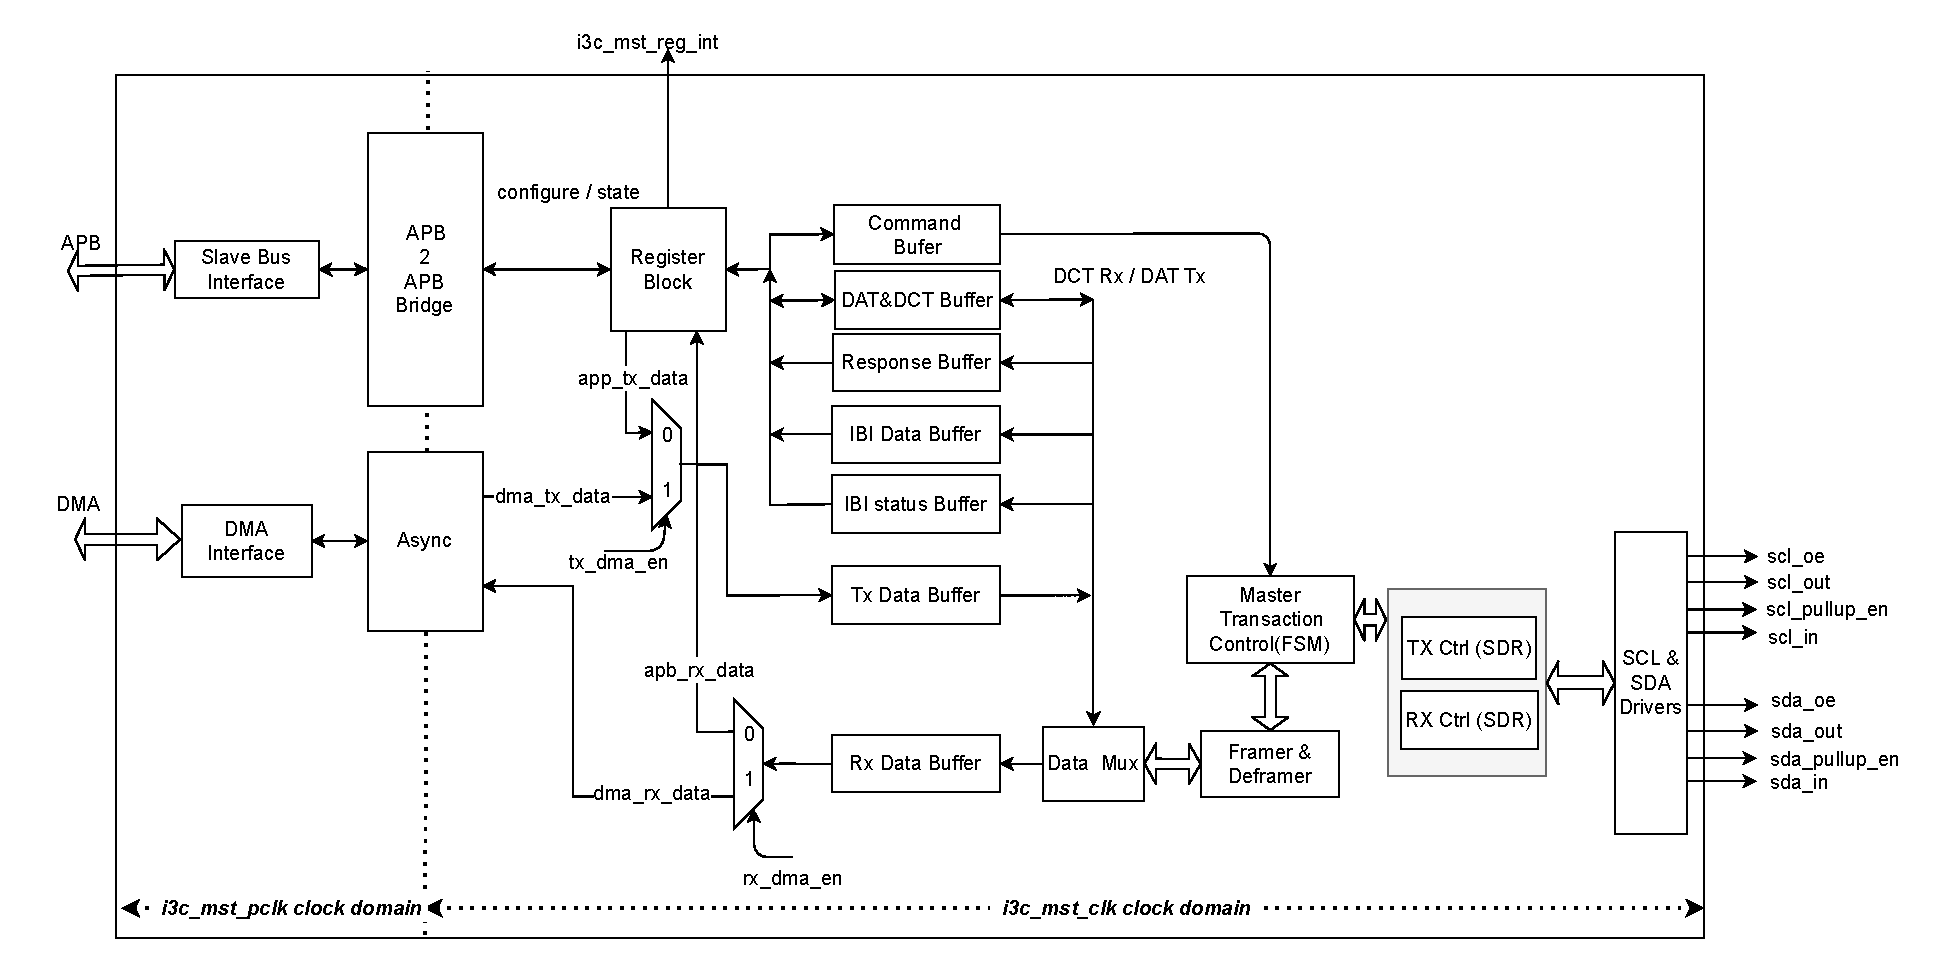
\includegraphics[width=1.0\linewidth]{47-I3C//figures/47-I3C_BlockDiagram__EN}
    \caption{I3C 控制器框图}
    \label{fig:i3c_mst_digram}
\end{figure}



I3C 控制器分为 APB 时钟域（即 i3c\_mst\_pclk clock domain）和核心时钟域（即 i3c\_mst\_core\_clk clock domain）。图 \ref{fig:i3c_mst_digram} 显示了 \chipname{} I3C 控制器的结构，包括：

\begin{itemize}
    \item DMA 接口：根据异步 FIFO 的占用情况，发出和撤销 AHB GDMA 的握手信号。
    \item 异步模块和 APB 桥：保持 APB 时钟和核心时钟之间的一致性。
    \item 寄存器块 (Register Block)：用于配置控制器的工作模式（如 I2C 兼容模式和 I3C 专用模式），并启用或禁用相关中断。同时作为数据传输接口，负责发送命令、动态地址表及写入数据，并接收设备特性表、读取数据及控制器状态响应。
    \item 命令缓冲区 (Command Buffer)：存储用于启动指定传输的命令。
    \item DAT (Device Address Table) 缓冲区：存储 I3C 目标的动态地址以及传统 I2C 设备的静态地址，这些地址用于识别总线上的不同设备并进行通信。
    \item DCT (Device Characteristics Table) 缓冲区：存储从 I3C 目标设备返回的设备特性信息。
    \item 响应缓冲区 (Response Buffer)：存储 I2C 或 I3C 传输的响应和状态信息。
    \item IBI 数据缓冲区 (IBI Data Buffer)：存储目标设备通过带内中断（IBI）上报的数据。
    \item IBI 状态缓冲区 (IBI Status Buffer)：在带内中断触发时存储状态信息。
    \item 发送数据缓冲区 (Tx Data Buffer)：存储待传输的数据。
    \item 接收数据缓冲区 (Rx Data Buffer)：存储接收到的数据。
    \item 数据多路复用器 (Data Mux)：选择发送数据的来源并确定接收数据的目标。
    \item 帧处理器和解帧处理器 (Framer and Deframer)：用于打包和拆分来自事务层和缓冲区控制器的数据。
    \item 发送控制 (TX Ctrl)：从帧处理器传输数据到总线上。
    \item 接收控制 (RX Ctrl)：从 SDA 线接收数据。
    \item 主事务控制 (FSM)：
    \begin{itemize}
      \item 执行命令缓冲区中预配置的数据传输指令。
      \item 生成符合 I3C 协议的时序序列，确保数据传输和接收的正确同步。
      \item 控制发送数据的帧处理和接收数据的解帧处理，保持传输过程中的数据完整性。
      \item 控制发送控制或接收控制模块在 SDA 管脚上传输或接收数据，协调总线上的整体数据流。
    \end{itemize}
\end{itemize}




%%%%%%%%%%%%%%%%%%%%%%%%%%%%%%
%%% Functional Description %%%
%%%%%%%%%%%%%%%%%%%%%%%%%%%%%%
\section{功能描述}
\label{sec:i3c-func-descr}

\subsection{时钟配置}

I3C 主时钟（\texttt{i3c\_mst\_clk}）可选择三种不同的时钟源，这些时钟源决定了 I3C 串行时钟 (SCL) 的最大频率。SCL 的频率由所选主时钟通过分频产生。

主时钟源可通过 \hyperref[mod:resclk]{复位和时钟} 章节中的 \hyperref[fielddesc:HPSYSCLKRSTI3CMSTCLKSRCSEL]{HP\_SYS\_CLKRST\_I3C\_MST\_CLK\_SRC\_SEL} 进行选择。可用的时钟源如下：

\begin{itemize}
    \item XTAL\_40M\_CLK：适用于需要低功耗和中等数据传输速度的场景。
    \item REF\_120M\_CLK：适用于需要较高数据传输速率但不要求最高速率的应用。
    \item REF\_160M\_CLK：适用于对数据传输速率要求最高的应用，为高速应用提供最佳性能。
\end{itemize}

关于频率和选择机制的详细信息，请参阅\hyperref[mod:resclk]{复位和时钟}章节。


\subsection{数据结构}

I3C 控制器定义了以下数据结构：
\begin{itemize}
    \item 命令描述符数据结构
    \item 响应描述符数据结构
    \item IBI 描述符数据结构
    \item DAT 数据结构
    \item DCT 数据结构
\end{itemize}

\subsubsection{命令描述符数据结构}

I3C 控制器通过命令描述符发起 CCC 传输、私有传输和动态地址分配，该描述符通过 \hyperref[regdesc:I3CMSTMEMCOMMANDBUFPORTREG]{I3C\_COMMAND\_PORT\_REG} 写入命令缓冲区。所有命令描述符分为三种类型：

\begin{itemize}
    \item \textbf{地址分配}：用于动态地址分配。
    \item \textbf{常规传输}：用于 CCC 传输和私有数据传输。
    \item \textbf{即时数据传输}：仅用于写操作，不用于读传输。命令中直接包含要传输的数据，从而可在无需额外缓冲操作的情况下立即传输小批量数据。
\end{itemize}

如图 \ref{fig:cmd_structure} 所示，I3C 控制器为每种命令类型定义了一个 64 位命令描述符结构。每个描述符用于向 I3C 总线上的目标设备调度一个命令事务。

\textbf{COMMAND\_L} 字段表示描述符的低 32 位，定义各字段在低字中的排布方式；\textbf{COMMAND\_H} 字段表示高 32 位，定义各字段在高字中的排布方式。每种命令类型在结构表中占据一行进行描述。



\begin{figure}[H]
    \centering
    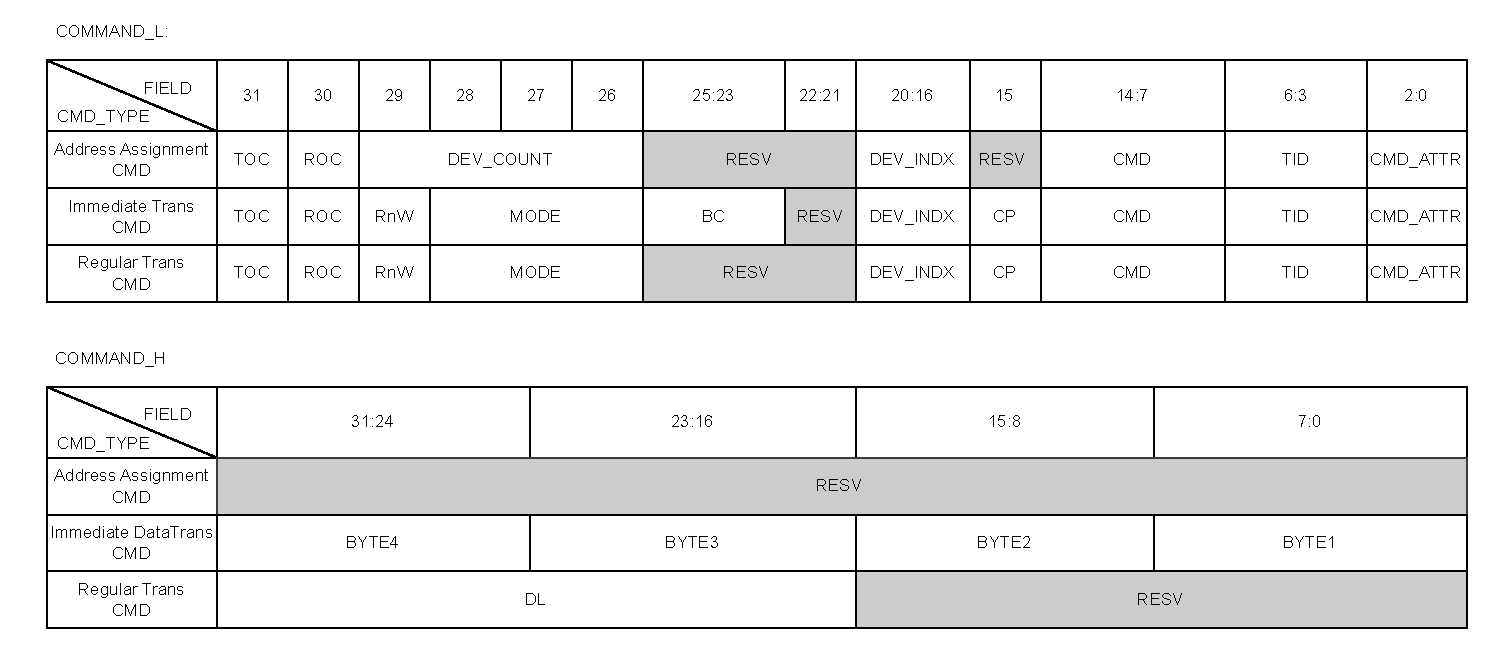
\includegraphics[width=1.0\linewidth]{47-I3C//figures/47-I3C_command_structure__EN}
    \caption{命令描述符数据结构}
    \label{fig:cmd_structure}
\end{figure}

命令描述符数据结构中每个字段的描述如下：
\begin{itemize}
    \item \textbf{CMD\_ATTR:}
    \begin{itemize}
        \item 0: 常规传输。通常用于一般 CCC 传输和私有数据传输场景。
        \item 1: 即时传输。适用于需要快速传输少量数据的情况，数据直接包含在命令中。
        \item 2: 地址分配。专门用于目标设备的动态地址分配操作。当新设备加入 I3C 总线时，I3C 控制器使用此模式为设备分配唯一地址。
    \end{itemize}
    \item \textbf{TID:} 事务 ID。用作此命令的标识标签。其值应在对应的 \textbf{响应描述符} 中保持一致。
    \item \textbf{CMD:} 传输命令的 CCC 值，用于指定 CCC 代码。
    \item \textbf{CP:} 命令存在标志。指示在 CCC 传输中 \textbf{CMD} 字段是否有效。
    \begin{itemize}
        \item 0: 此结构描述 SDR 传输，因此 CMD 字段无效。
        \item 1: 此结构描述 CCC 传输，因此 CMD 字段有效。
    \end{itemize}
    \item \textbf{DEV\_INDEX:} 指示本次传输所寻址的目标设备在 DAT 表中的索引位置。该索引处存储了对应目标设备的静态地址及寻址信息。在广播 CCC 传输中，此字段保留。
    \item \textbf{RESV:} 保留。
    \item \textbf{DEV\_COUNT:} 指示要分配动态地址的设备数量。
    \item \textbf{RnW:} 标识此传输的方向。
    \begin{itemize}
        \item 0: 写传输
        \item 1: 读传输
    \end{itemize}
    \item \textbf{BC}: 指示 COMMAND\_H 中的字节数。
    \item \textbf{MODE:} 数据传输速度和模式。设置 I3C 或 I2C 传输的模式和速度。此字段的解释取决于设备是在 I3C 模式还是 I2C 模式（参见由字段 DEV\_INDEX 索引的 DAT 表条目中的 DEVICE 字段）。\\
    I3C 模式的值：
    \begin{itemize}
        \item I3C SDR0: 标准 SDR 速度，其时序寄存器为 REG\_I3C\_PP\_LOW\_PERIOD 和 REG\_I3C\_PP\_HIGH\_PERIOD。
        \item I3C SDR1–4: 较低的 SDR 速度，其时序寄存器为 REG\_I3C\_EXT\_LOW\_PERIOD1–4。
    \end{itemize}
    I2C 模式的值：
    \begin{itemize}
        \item 0x0: I2C 快速模式，其时序寄存器为 REG\_I2C\_FM\_LOW\_PERIOD 和 REG\_I2C\_FM\_HIGH\_PERIOD。
        \item 0x1: I2C 快速模式增强（FM+），其时序寄存器为 REG\_I2C\_FMP\_LOW\_PERIOD 和 REG\_I2C\_FMP\_HIGH\_PERIOD。
    \end{itemize}
    \item \textbf{ROC:} 完成响应，控制在传输命令成功完成后是否发送响应状态。
    \begin{itemize}
        \item 0: 不需要响应状态。
        \item 1: 需要响应状态。
    \end{itemize}
    \item \textbf{TOC:} 完成终止，控制传输命令完成后发出的总线条件。对于 ENTDAA，此字段必须设置为 1。
    \begin{itemize}
        \item 0: 在传输结束时发出重复启动 (Sr)。
        \item 1: 在传输结束时发出停止 (P)。
    \end{itemize}
    \item \textbf{DL:} 数据长度，指示要传输的字节数。
    \item \textbf{BYTE1-4}: 即时数据传输的数据字节1–4。
\end{itemize}


\subsubsection{响应描述符数据结构}

响应描述符，如图 \ref{fig:resp-structure} 所示，是一个只读结构，用于描述传输命令是否成功以及传输的数据量。I3C 控制器使用此数据结构将传输命令的状态返回到响应缓冲区。可以通过 \hyperref[regdesc:I3CMSTMEMRESPONSEBUFPORTREG]{I3C\_MST\_RESP\_BUFFER\_PORT\_REG} 读取响应描述符。

\begin{figure}[H]
    \centering
    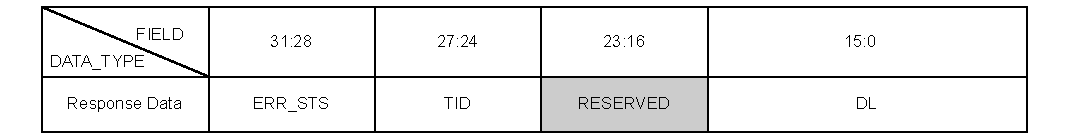
\includegraphics[width=1\linewidth]{47-I3C//figures/47-I3C_RESP_STRUCTURE__EN}
    \caption{响应描述符数据结构}
    \label{fig:resp-structure}
\end{figure}

响应描述符结构中的每个字段描述如下：
\begin{itemize}
    \item \textbf{DL}，数据长度。此字段的含义取决于上下文：
    \begin{itemize}
        \item 对于写传输：剩余数据长度（以字节为单位）
        \item 对于读传输：接收的数据长度（以字节为单位）
        \item 对于地址分配：剩余设备数量
    \end{itemize}
    \item \textbf{TID}，命令的识别标签。此值必须与总线上发送的命令之一匹配。取值范围：
    \begin{itemize}
        \item 0 \verb+~+ 15：有效事务 ID
    \end{itemize}
    \item \textbf{ERR\_STS}，错误类型。指示响应状态，成功或处理命令时遇到的错误类型。
    \begin{itemize}
        \item 0：无错误
        \item 1 \verb+~+ 2：保留
        \item 3：读取数据长度不匹配
        \item 4：I3C 广播地址 NACK 错误
        \item 5：地址 NACK 或动态地址分配 NACK
        \item 6：接收数据缓冲区溢出/发送数据缓冲区欠载
        \item 7 \verb+~+ 8：保留
        \item 9：I2C 从设备写入数据 NACK 错误
        \item 10 \verb+~+ 15：保留
    \end{itemize}
\end{itemize}

\subsubsection{IBI 状态描述符数据结构}

IBI 状态描述符，如图 \ref{fig:ibi-data-structure} 所示，是一个只读结构，用于描述从 I3C 总线上的目标设备接收到的 IBI 事件。I3C 控制器使用此数据结构将接收到的带内中断 (IBI) 的状态返回到 IBI 缓冲区。可以通过 \hyperref[regdesc:I3CMSTMEMIBISTATUSBUFREG]{I3C\_MST\_MEM\_IBI\_STATUS\_BUF\_REG} 读取 IBI 描述符。

\begin{figure}[H]
    \centering
    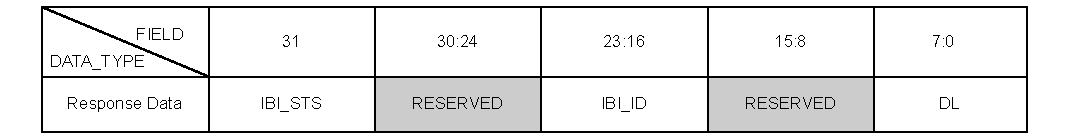
\includegraphics[width=1\linewidth]{47-I3C//figures/47-I3C_IBI_STRUCTURE__EN}
    \caption{IBI 状态描述符数据结构}
    \label{fig:ibi-data-structure}
\end{figure}

IBI 状态描述符数据结构中的每个字段描述如下：

\begin{itemize}
    \item \textbf{DL}，数据长度。接收到的 IBI 数据中的数据字节数。
    \item \textbf{IBI\_ID}，在 START 之后接收到的 IBI 标识符，包含目标设备的设备地址和读/写位。
    \item \textbf{IBI\_STS}，IBI 状态。
    \begin{itemize}
        \item 0：IBI ACK。该 IBI 以 ACK 处理。
        \item 1：IBI NACK。该 IBI 以 NACK 处理。
    \end{itemize}
\end{itemize}

\subsubsection{DAT 数据结构}

DAT 表用于存储连接到 I3C 总线的设备地址，以及每个设备的多个控制和信息字段。软件将这些数据结构填充到 DAT 表中，如图 \ref{fig:dat_i3c_dyn_sta} 和图 \ref{fig:dat_i2c_ds} 所示。DAT 表条目由命令描述符中的 DEV\_INDEX 字段索引，控制器在动态地址分配及其他传输操作中通过该索引访问对应的设备信息。

可以通过软件编程的动态地址值为目标设备的 IBI 设置每个设备的优先级。

设备地址表支持以下三种类型的数据结构：

\begin{itemize}
\item 第一种类型如图 \ref{fig:dat_i3c_dyn_sta} 所示，适用于具有静态地址的 I3C 设备。
    \begin{itemize}
         \item \textbf{静态地址}：I3C 目标的静态地址。
         \item \textbf{动态地址}：
         \begin{itemize}
             \item 如果通过 SETDASA CCC 用于地址分配，则是要分配给具有静态地址的 I3C 设备的动态地址。
             \item 对于其他传输，动态地址用作目标的地址。
         \end{itemize}
         \item \textbf{DNRC}：设备 NACK 重试计数器。它决定当前传输被拒绝时的重试次数。
         \item \textbf{Bit[31]}：0。表示 I3C 设备。
    \end{itemize}

\begin{figure}[H]
    \centering
    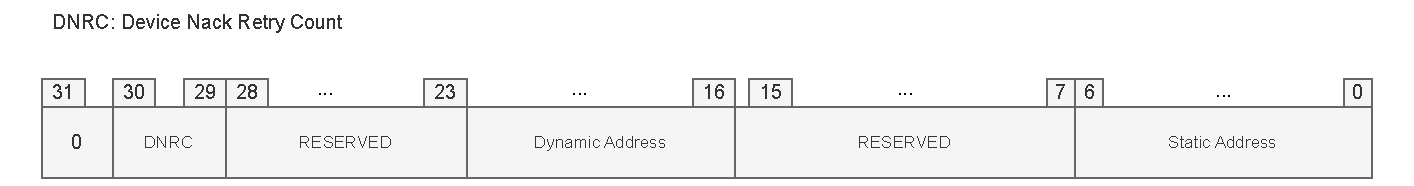
\includegraphics[width=1\linewidth]{47-I3C//figures/47-I3C_DAT_I3C_DYN_STA}
    \caption{具有静态地址的 I3C 目标设备的 DAT 结构}
    \label{fig:dat_i3c_dyn_sta}
\end{figure}

\item 第二种类型如图 \ref{fig:dat_i3c_only_dyn} 所示，适用于具有动态地址的纯 I3C 设备。
      \begin{itemize}
       \item \textbf{动态地址}：
             \begin{itemize}
                 \item 如果通过 ENTDAA CCC 用于地址分配，则是要分配给没有静态地址的 I3C 设备的动态地址。
                 \item 对于其他传输，动态地址用作目标的地址。
             \end{itemize}
       \item \textbf{PAR}：7 位动态地址的奇偶校验位。
       \item \textbf{DNRC}：设备 NACK 重试计数器。它决定当前传输被拒绝时的重试次数。
       \item \textbf{Bit[31]}：0。表示 I3C 设备。
     \end{itemize}
\end{itemize}

\begin{figure}[H]
    \centering
    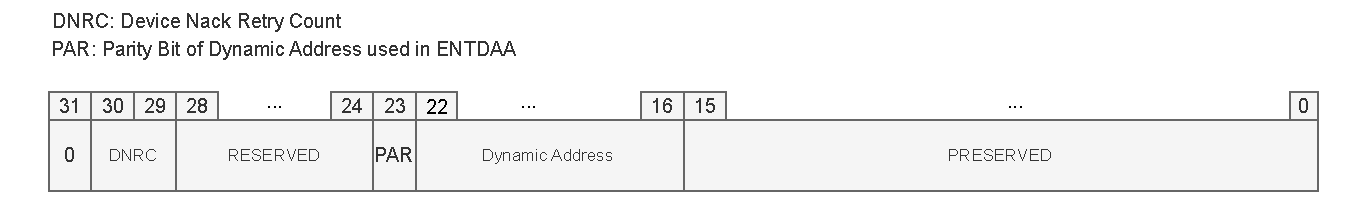
\includegraphics[width=1\linewidth]{47-I3C//figures/47-I3C_DAT_I3C_ONLY_DYN}
    \caption{没有静态地址的纯 I3C 目标设备的 DAT 数据结构}
    \label{fig:dat_i3c_only_dyn}
\end{figure}
\begin{itemize}

\item 第三种类型如图 \ref{fig:dat_i2c_ds} 所示，适用于具有静态地址的 I2C 设备。
      \begin{itemize}
       \item \textbf{静态地址}：I2C 设备的静态地址。
       \item \textbf{DNRC}：设备 NACK 重试计数器。它决定当前传输被拒绝时的重试次数。
       \item \textbf{Bit[31]}：1。表示 I2C 设备。
     \end{itemize}
\end{itemize}
\begin{figure}[H]
    \centering
    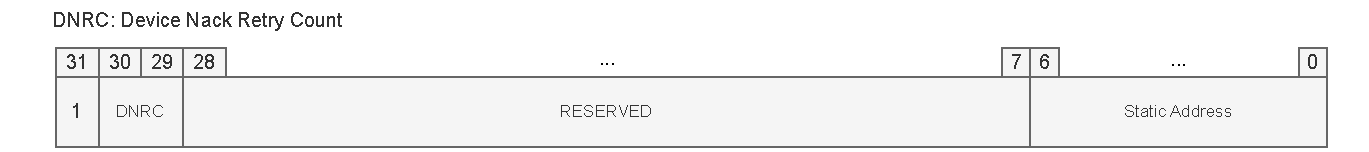
\includegraphics[width=1\linewidth]{47-I3C//figures/47-I3C_DAT_I2C_DS}
    \caption{I2C 从设备的 DAT 数据结构}
    \label{fig:dat_i2c_ds}
\end{figure}

\subsubsection{DCT 数据结构}

DCT 表记录 I3C 总线上参与动态地址分配 (ENTDAA) 过程的每个设备的设备特性 (PID、BCR、DCR) 和分配的动态地址。I3C 控制器接收由 ENTDAA 传输的字节，按它们在总线上出现的顺序接收。默认情况下，接收到的第一个位存储在最低有效位位置。在字数据存储模式下，遵循小端字节序惯例，即先接收的字节存储在字的低地址部分（低索引位置），随后接收的字节按顺序存储在高地址方向，以形成完整的字数据。如图 \ref{fig:dct_structure} 所示，DCT 中每个设备包含四个条目。

\begin{figure}[H]
    \centering
    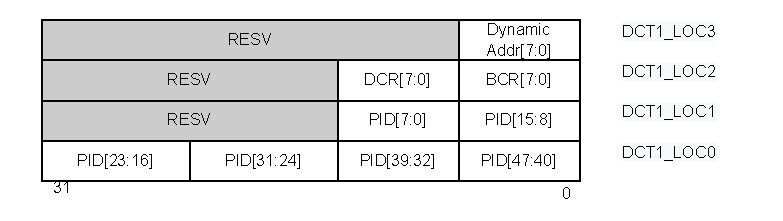
\includegraphics[width=0.8\linewidth]{47-I3C//figures/47-I3C_DCT}
    \caption{DCT 数据结构}
    \label{fig:dct_structure}
\end{figure}

\subsection{数据转换}

RX Ctrl 和 TX Ctrl 中的数据移位器负责串行/并行转换。它将 TX 数据缓冲区中的字节数据转换为输出的串行比特流，或将输入的串行比特流转换为 DCT 表、RX 数据缓冲区和 IBI 数据缓冲区中的字节数据。
\begin{itemize}
    \item 配置 \hyperref[fielddesc:I3CMSTREGRXBITORDER]{I3C\_MST\_REG\_RX\_BIT\_ORDER} 以选择接收比特的存储顺序。
    \item 配置 \hyperref[fielddesc:I3CMSTREGRXBYTEORDER]{I3C\_MST\_REG\_RX\_BYTE\_ORDER} 以选择小端或大端格式。
\end{itemize}

\subsection{DAT 和 DCT 内存控制}

DCT 表对 I3C 控制器而言是只写不可读，对 CPU 则是只读不可写。DAT 表对 CPU 是只写不可读，对 I3C 控制器则是只读不可写。DAT 表和 DCT 表共享一块 60×32 位的 RAM，其中前 48 个条目（偏移地址 0～47）分配给 DCT 表，后 12 个条目（偏移地址 48～59）分配给 DAT 表。


如图 \ref{fig:dct_dat_ram} 所示，此 RAM 中的每个条目映射到一个 CPU 可访问的唯一端口寄存器：

\begin{itemize}
    \item DAT 表：\hyperref[regdesc:I3CMSTMEMDEVADDRTABLENLOCREG]{I3C\_MST\_MEM\_DEV\_ADDR\_TABLE\regindex{n}\_LOC\_REG}（\regindex{n}: 1～12）
    \item DCT 表：\hyperref[regdesc:I3CMSTMEMDEVCHARTABLENLOCMREG]{I3C\_MST\_MEM\_DEV\_CHAR\_TABLE\regindex{n}\_LOC\regindex{m}\_REG}（\regindex{n}: 1～12，\regindex{m}: 1～4）
\end{itemize}
\begin{figure}[H]
    \centering
    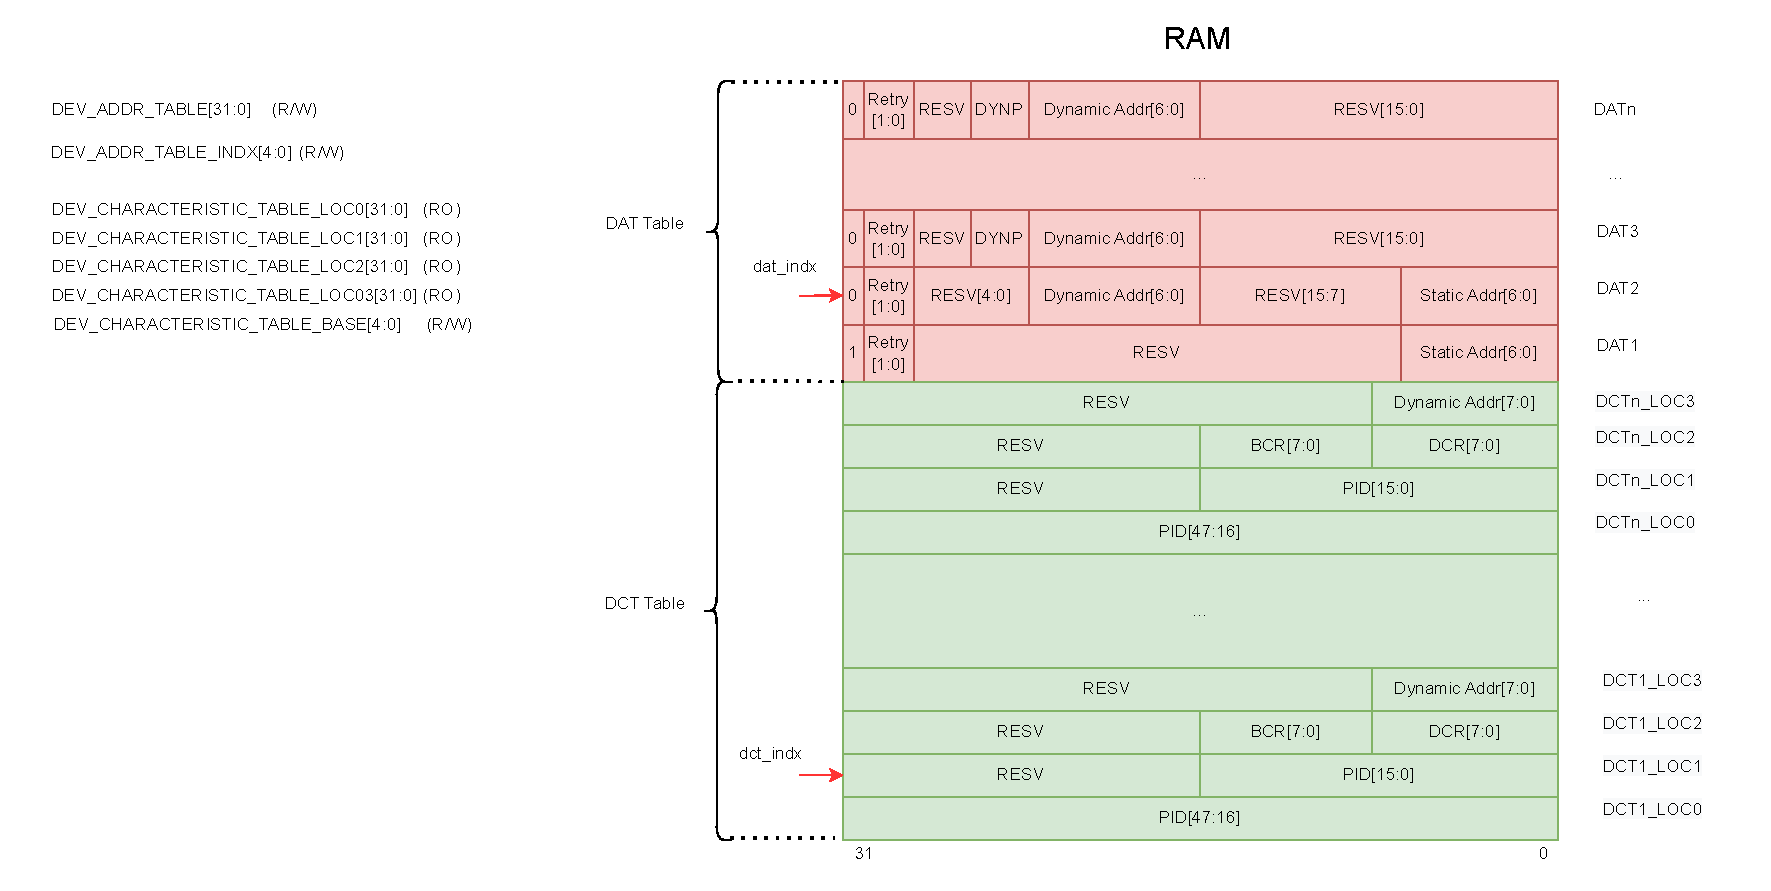
\includegraphics[width=1.0\linewidth]{47-I3C/figures/47-I3C_DAT_DCT_BUF}
    \caption{DAT 和 DCT 共享 RAM}
    \label{fig:dct_dat_ram}
\end{figure}

在使用 ENTDAA CCC 进行动态地址分配期间，dat\_indx 和 dct\_indx 分别表示 DAT 缓冲区和 DCT 缓冲区中的位置，I3C 控制器在这些位置存储赢得仲裁的目标设备的动态地址和设备特性。可通过 \hyperref[regdesc:I3CMSTDEVICETABLEREG]{I3C\_MST\_DEVICE\_TABLE\_REG} 中的 R/W 字段 \hyperref[fielddesc:I3CMSTREGDATDAAINITINDEX]{I3C\_MST\_REG\_DAT\_DAA\_INIT\_INDEX} 和 \hyperref[fielddesc:I3CMSTREGDCTDAAINITINDEX]{I3C\_MST\_REG\_DCT\_DAA\_INIT\_INDEX} 分别配置 dat\_indx 和 dct\_indx 的初始值。

地址分配结束后，可通过 \hyperref[regdesc:I3CMSTDEVICETABLEREG]{I3C\_MST\_DEVICE\_TABLE\_REG} 中的 RO 字段 \hyperref[fielddesc:I3CMSTPRESENTDATINDEX]{I3C\_MST\_PRESENT\_DAT\_INDEX} 和 \hyperref[fielddesc:I3CMSTPRESENTDCTINDEX]{I3C\_MST\_PRESENT\_DCT\_INDEX} 分别读取当前的 dat\_indx 和 dct\_indx 值。

\subsection{TX/RX 数据存储}

TX 数据缓冲区（TX Data Buffer）和 RX 数据缓冲区（RX Data Buffer）均为 32×32 位，并以 FIFO 模式工作。TX 数据缓冲区对 CPU 或 AHB GDMA 为只写（可通过设置 \hyperref[fielddesc:I3CMSTREGDMATXEN]{I3C\_MST\_REG\_DMA\_TX\_EN} 启用 DMA TX 功能），对 I3C 控制器为只读。它按传输顺序存储来自 CPU 或 AHB DMA 的数据。在常规写传输过程中，I3C 控制器从 TX 数据缓冲区读取指定长度的数据，并通过 SDA 线按顺序发送。CPU 可通过 \hyperref[fielddesc:I3CMSTMEMTXDATAPORT]{I3C\_MST\_MEM\_TX\_DATA\_PORT} 向 TX 数据缓冲区写入数据。

RX 数据缓冲区对控制器为只写，对 CPU 或 AHB GDMA 为只读（可通过设置 \hyperref[fielddesc:I3CMSTREGDMARXEN]{I3C\_MST\_REG\_DMA\_RX\_EN} 启用 DMA RX 功能）。它按照 \hyperref[fielddesc:I3CMSTREGRXBITORDER]{I3C\_MST\_RX\_BIT\_ORDER} 和 \hyperref[fielddesc:I3CMSTREGRXBYTEORDER]{I3C\_MST\_RX\_BYTE\_ORDER} 指定的顺序存储从 SDA 接收到的数据。

TX 和 RX 数据缓冲区每次最多可存储 128 字节。对于超过 128 字节的传输，必须根据 \hyperref[int:TXDATABUFTHLDINT]{TX\_DATA\_BUF\_THLD\_INT} 及时填充 TX 缓冲区，并根据 \hyperref[int:RXDATABUFTHLDINT]{RX\_DATA\_BUF\_THLD\_INT} 及时读取 RX 缓冲区。TX 阈值必须确保在 TX 缓冲区清空前完成填充，RX 阈值必须确保在 RX 缓冲区满之前完成读取，否则传输将失败。

\subsection{DMA 模式}

当 I3C 控制器发送和接收大量数据时，建议使用直接内存访问（DMA）模式以提高效率。要正确使用 DMA，请按以下步骤配置并注意相应行为：

\begin{enumerate}
    \item 启用 DMA 通道：
    \begin{itemize}
        \item 配置 \texttt{I3C\_MST\_REG\_DMA\_TX\_EN} 和 \texttt{I3C\_MST\_REG\_DMA\_RX\_EN}，分别启用 TX（发送）和 RX（接收）通道；
        \item 注意：DMA 仅传输数据，不会传输命令或状态信息。
    \end{itemize}

    \item CPU 缓存命令并配置链表：
    \begin{itemize}
        \item 启用 DMA TX 和 RX 模式后，CPU 必须首先将命令缓存到命令缓冲区中。
        \item 根据需要配置 AHB GDMA（高级高性能总线通用 DMA）的发送和接收链表。
        \item 配置完成后，开始数据传输。此时，AHB GDMA 与 I3C 控制器协同工作完成数据的发送和接收。
    \end{itemize}

    \item 配置 AHB GDMA：
    \begin{itemize}
        \item 配置接收（RX）通道：
        \begin{itemize}
            \item 在 RX 开始接收之前，配置接收链表；
            \item 将 \texttt{GDMA\_INLINK\_ADDR\_CHn} 指向第一个接收链表描述符，并设置 \texttt{GDMA\_INLINK\_START\_CHn}；
            \item 启动后，I3C 控制器将接收到的数据传给 AHB GDMA，AHB GDMA 会把数据存入链表指定位置。
        \end{itemize}

        \item 配置发送（TX）通道：
        \begin{itemize}
        \item 在 TX 开始发送之前，准备发送链表和要发送的数据；
        \item 将 \texttt{GDMA\_OUTLINK\_ADDR\_CHn} 指向第一个发送链表描述符，并设置 \texttt{GDMA\_OUTLINK\_START\_CHn}；
        \item 启动后，GDMA 引擎从发送链表指定的位置读取数据，并将其发送到 I3C 控制器。I3C 控制器随后通过 SDA 线传输数据。
        \end{itemize}
    \end{itemize}

    \item 数据长度与对齐规则：
    \begin{itemize}
        \item 发送/接收的数据长度由命令描述符中的“数据长度”字段决定；
        \item I3C 控制器与 AHB GDMA 以字（word）为单位交互，传输为字对齐；
        \item 当“数据长度”不是字的整数倍时：在 RX 方向，I3C 控制器会自动用 0 填充以实现字对齐；在 TX 方向，AHB GDMA 可填充无效数据，I3C 控制器只根据“数据长度”提取并发送有效字节，不会发送填充的无效字节。
    \end{itemize}
\end{enumerate}

\subsection{传输类型}

I3C 控制器是一个仅支持 SDR 的外设，遵循总线通信协议在控制器和目标设备之间传输数据。

\subsubsection{动态地址分配（DAA）}

作为控制器，I3C 控制器执行动态地址分配（DAA）程序，为连接到 I3C 总线的每个 I3C 设备提供一个唯一的动态地址。一旦设备接收到动态地址，在所有后续事务中都会使用该分配的动态地址，直到控制器更改这个动态地址。

如图\ref{fig:daa_trans_format}所示，有两种 DAA 方法：
\begin{itemize}
    \item SETDASA
    \item ENTDAA
\end{itemize}
\begin{figure}[H]
    \centering
    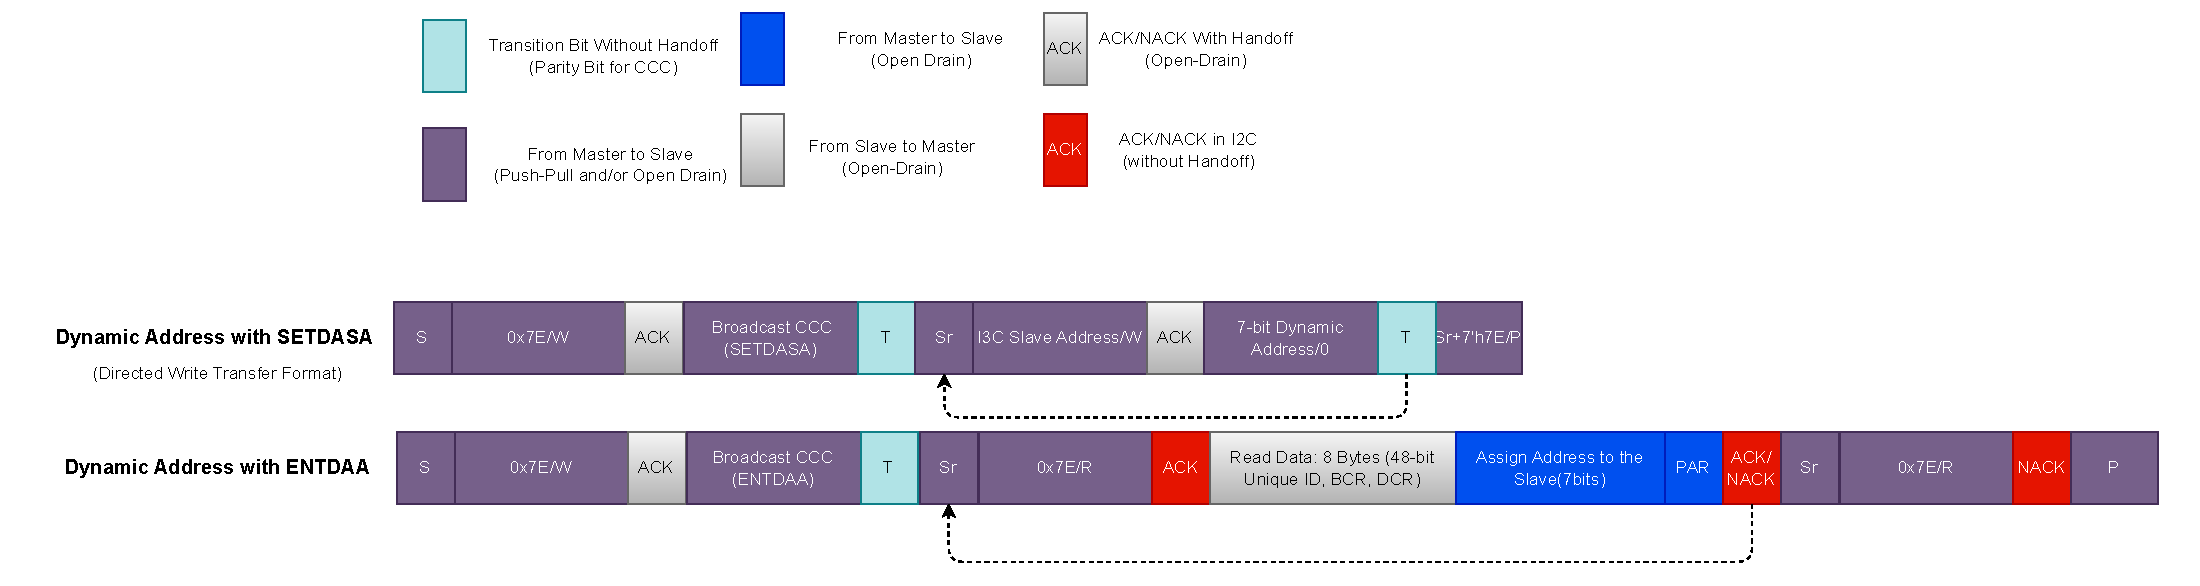
\includegraphics[width=1\linewidth]{47-I3C/figures/47-I3C_DAA}
    \caption{地址分配传输格式}
    \label{fig:daa_trans_format}
\end{figure}

\subparagraph{SETDASA 过程}

SETDASA 是一个定向的通用命令代码，允许控制器为任何具有已知静态地址的 I3C 设备分配动态地址。此方法比使用 ENTDAA 过程更快。

\subparagraph{ENTDAA 过程}

控制器通过发送广播型的 ENTDAA 公共命令码（CCC），为尚未分配动态地址的 I3C 设备分配动态地址。该过程在系统冷启动之后执行，并在对具有静态地址的设备完成 SETDASA 动态地址分配流程后进行。

控制器可以通过一次或多次 ENTDAA 命令，为所有已连接的 I3C 设备完成动态地址分配。每条 ENTDAA 命令可分配的设备数量受 DAT 表和 DCT 表深度的限制，最多可支持 12 个设备。

\subsubsection{CCC 传输}

公共命令码（CCC）是所有 I3C 目标设备均支持的全局命令，可直接发送给某个特定 I3C 目标设备，也可同时广播给所有目标设备。

命令码空间分为广播命令和直接命令：
\begin{itemize}
\item 广播 CCC 命令的命令码范围为 0x00 到 0x7F
\item 直接 CCC 命令的命令码范围为 0x80 到 0xFE
\end{itemize}

所有 CCC 命令均以 I3C 广播地址（7 位地址 0x7E）开头。也就是说，在 START 或 Repeated START 之后，CCC 命令的地址始终为 0x7E，且 RnW 位始终为写入。

\subparagraph{直接 CCC 传输}

直接 CCC 传输格式如图 \ref{fig:i3c_trans_format} 所示。直接写 CCC（Direct Write CCC）根据目标设备的动态地址，将指令发送给一个或多个特定的 I3C 目标设备。直接读 CCC（Direct Read CCC）则根据目标设备的动态地址，从一个或多个特定的 I3C 目标设备读取数据。所有直接 CCC 命令均以 STOP 或 Repeated START 结束，之后使用 I3C 广播地址（0x7E）。
\subparagraph{广播 CCC 传输}

广播 CCC 传输格式如图 \ref{fig:i3c_trans_format} 所示。广播写 CCC (Broadcast Write CCC) 会被所有 I3C 目标设备接收。所有广播写 CCC 命令都以 Repeated START 或 STOP 结束，但 ENTDAA 除外，它始终以 STOP 结束。

\begin{figure}[H]
    \centering
    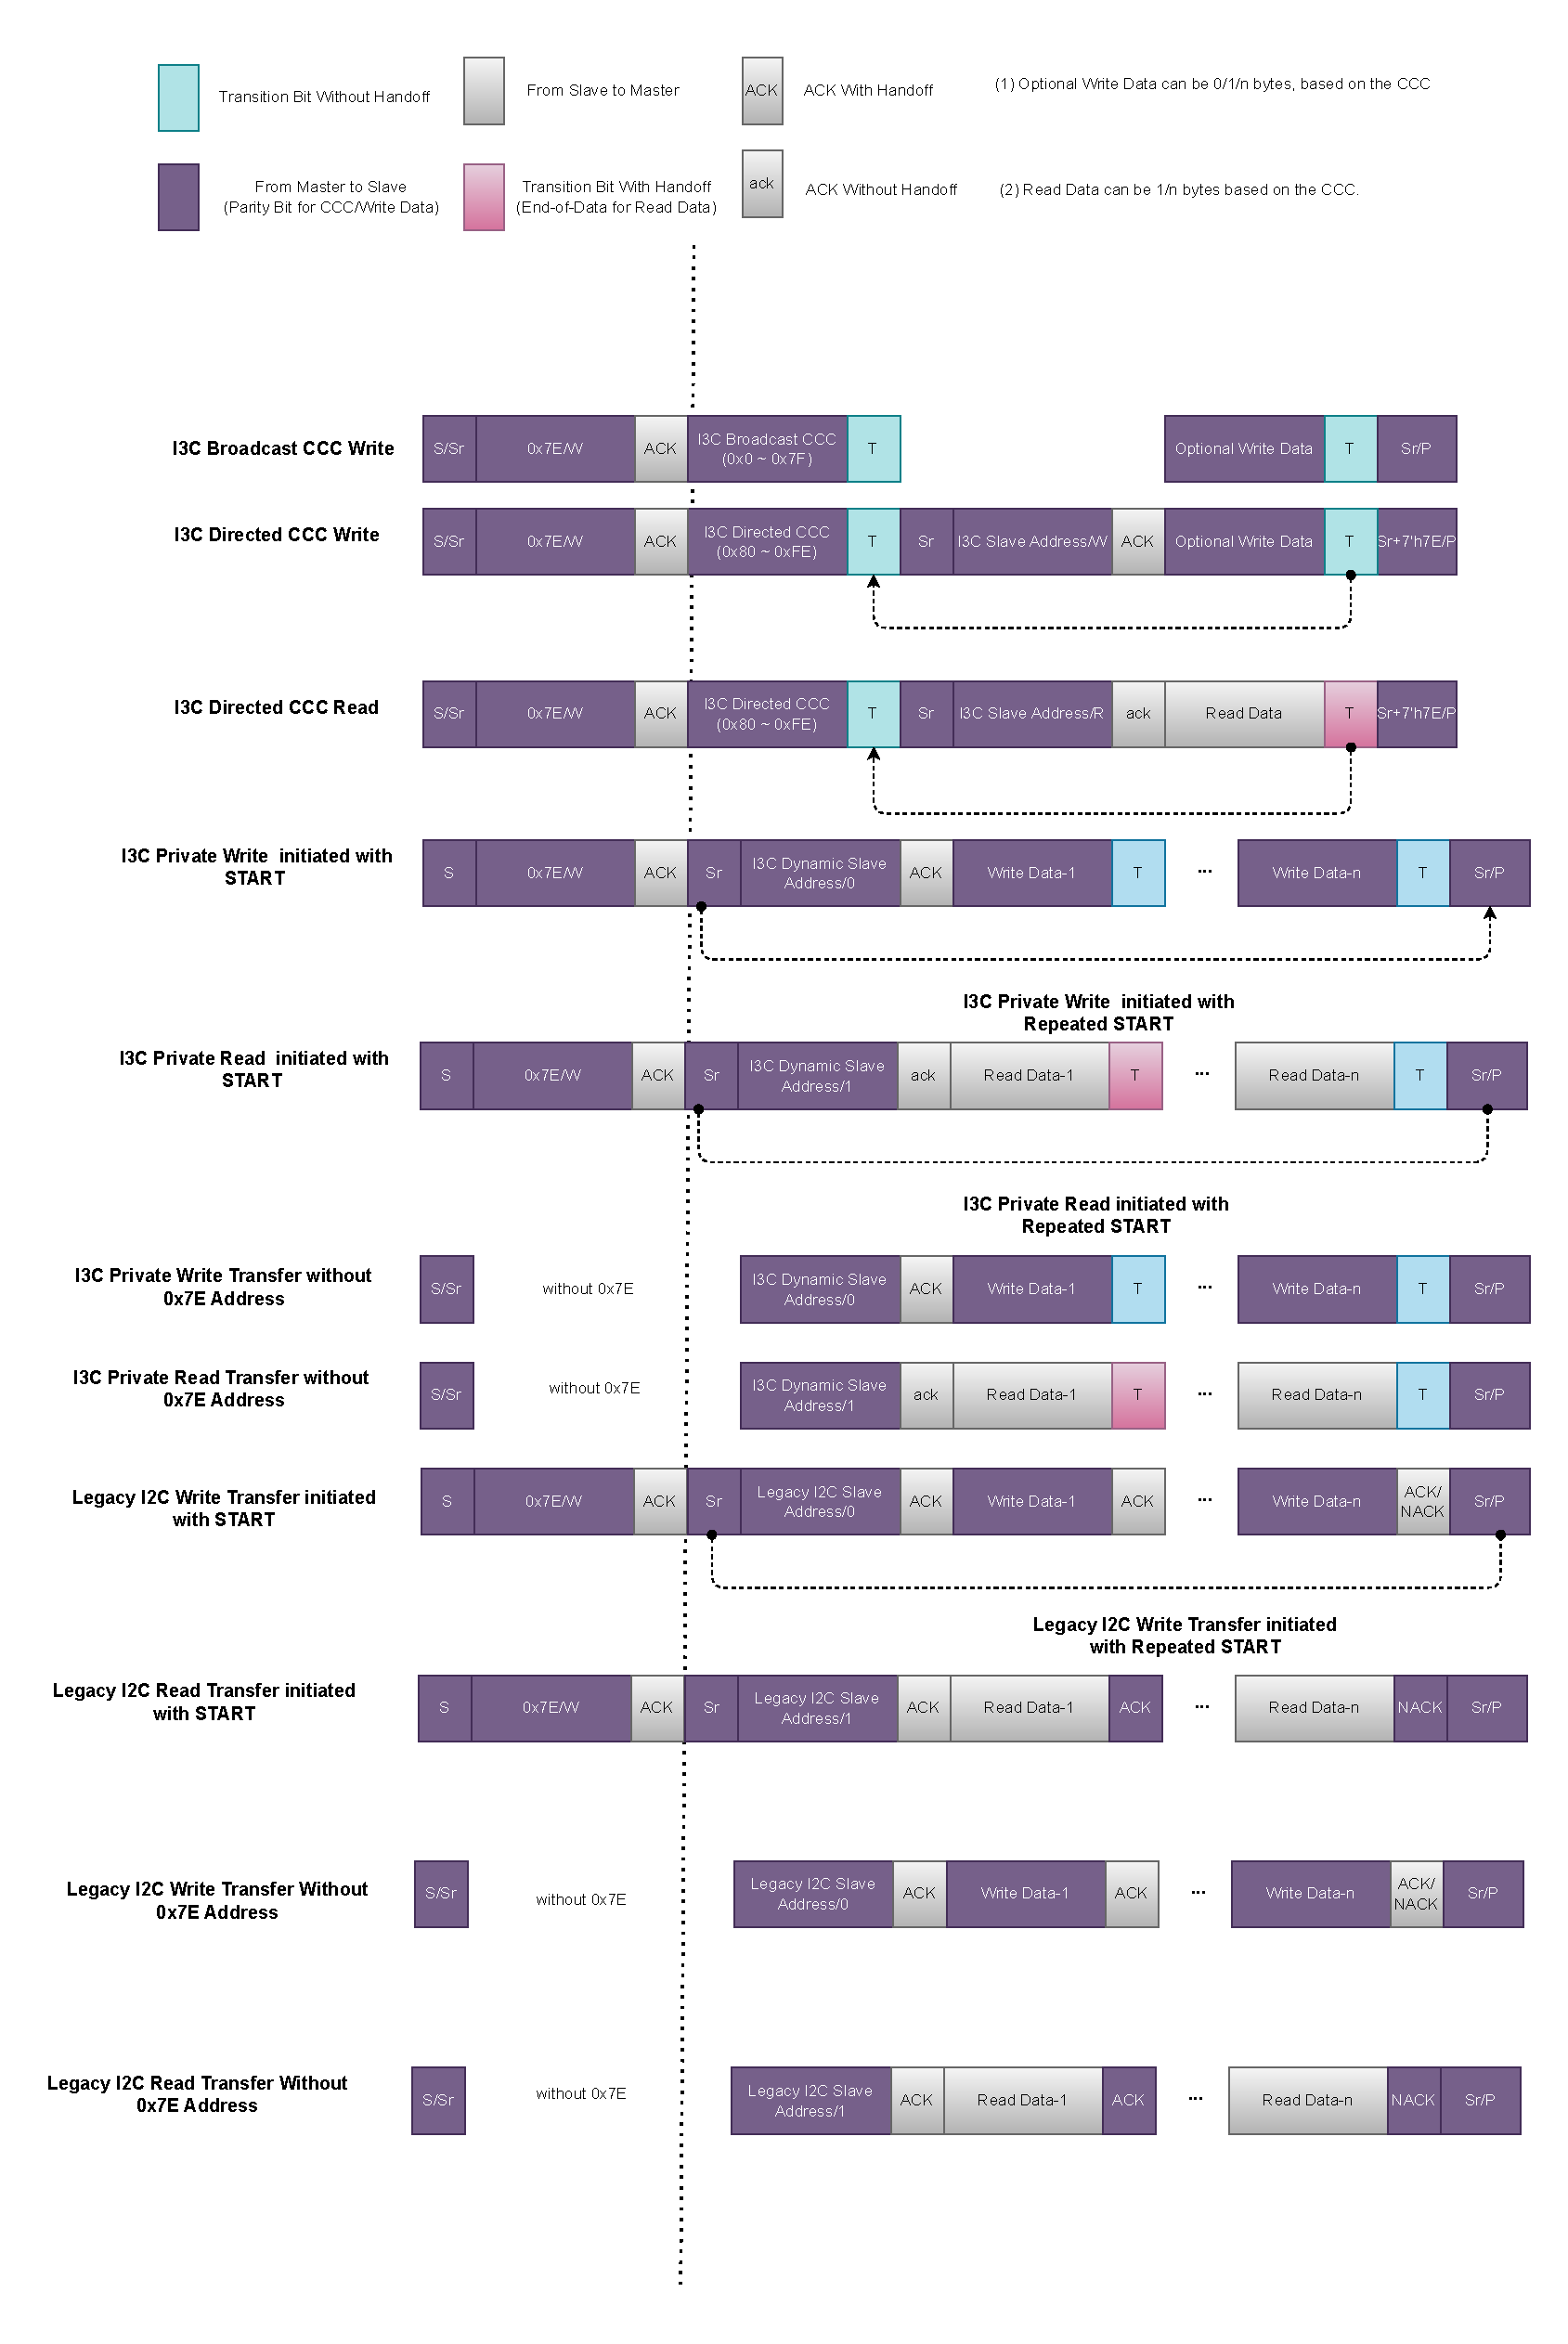
\includegraphics[width=0.8 \linewidth]{47-I3C//figures/47-I3C_Format}
    \caption{I3C 传输格式}
    \label{fig:i3c_trans_format}
\end{figure}

\subsubsection{私有数据传输}

如图 \ref{fig:i3c_trans_format} 所示，I3C 可以像 I2C 一样发起无需 CCC 的私有传输。如果将 \hyperref[fielddesc:I3CMSTREGBAINCLUDE]{I3C\_MST\_BA\_INCLUDE} 设置为 1，I3C 控制器可以在私有传输中包含广播地址头。如果未包含广播地址，则从目标设备发起的 IBI 可能无法赢得仲裁，从而延迟 IBI 的接收。

\subsubsection{传统 I2C 传输}

I3C 控制器使用 I2C 协议对传统 I2C 设备发起 I2C 传输。通过设置 \hyperref[fielddesc:I3CMSTREGBAINCLUDE]{I3C\_MST\_BA\_INCLUDE}，I3C 控制器可以在 I2C 传输中包含广播地址头，从而允许来自 I3C 设备的 IBI 获得优先权。

\subsubsection{带内中断 (IBI) 处理}

I3C 控制器仅支持目标设备中断请求 (SIR)，这是一种独特的类型（分配的动态地址设置了读取标志）。I3C 控制器中有两个 32 位向量控制寄存器：

\begin{itemize}
    \item \hyperref[regdesc:I3CMSTIBISIRREQREJECTREG]{I3C\_MST\_SIR\_REQ\_REJECT}：单独控制每个 I3C 目标设备的响应。
    \item \hyperref[regdesc:I3CMSTIBISIRREQPAYLOADREG]{I3C\_MST\_SIR\_REQ\_PAYLOAD}：指示在 I3C 目标设备发起的 IBI 请求之后，是否还会紧跟一个 IBI 负载。
\end{itemize}

上述寄存器中的每个位通过模运算映射到总线上分配给 I3C 目标设备的唯一动态地址，映射关系如下式所示。

这种模运算限制了 I3C 目标设备的动态地址范围，但允许 I3C 控制器灵活地处理来自各种 I3C 目标设备的带内中断。具体而言，动态地址与寄存器位的对应关系由下式给出：

\textbf{IBI\_Index = mod32\{IBI\_DYNAMIC\_ADDR[6:5]+IBI\_DYNAMIC\_ADDR[4:0]\}}\\

SIR\_x 是寄存器中的一位，假定在模运算后映射到 I3C 目标设备 I3C\_SLV\_y。

\subparagraph{ACK SIR}
当 \hyperref[regdesc:I3CMSTIBISIRREQREJECTREG]{I3C\_MST\_SIR\_REQ\_REJECT} 中的 SIR\_x 设置为 0 时，I3C 控制器对来自 I3C\_SLV\_y 的 SIR 请求返回 ACK，并在 IBI 状态缓冲区中生成 IBI 状态响应以通知应用程序。如果 \hyperref[regdesc:I3CMSTIBISIRREQPAYLOADREG]{I3C\_MST\_SIR\_REQ\_PAYLOAD} 中的 SIR\_x 设置为 1，I3C 控制器还会接收紧跟 SIR 后面的强制字节到 IBI 数据缓冲区中。

\subparagraph{NACK SIR}
当 \hyperref[regdesc:I3CMSTIBISIRREQREJECTREG]{I3C\_MST\_SIR\_REQ\_REJECT} 中的 SIR\_x 设置为 1 时，I3C 控制器对来自 I3C\_SLV\_y 的 SIR 请求响应 NACK。如果 \hyperref[fielddesc:I3CMSTREGAUTODISIBIEN]{I3C\_MST\_AUTO\_DIS\_IBI\_EN} 设置为 1，则在该 SIR 被 NACK 之后，I3C 控制器可以向发起 SIR 的设备发送一条定向的 DISEC CCC。

如果 \hyperref[fielddesc:I3CMSTREGIBIRSTARTTRANSEN]{I3C\_MST\_IBI\_RSTART\_TRANS\_EN} 设置为 1，I3C 控制器在 IBI 完成后继续执行之前被 IBI 中断的命令。

\subsection{时序配置}
I3C 控制器提供了一组时序配置寄存器，软件可基于 I3C 主时钟（i3c\_mst\_clk）精确配置 SCL 时钟波形、SDA 数据建立/保持时序以及总线条件（START、STOP、Bus Free）时序。

\subsubsection{计数单位约定}
所有时序寄存器均以 i3c\_mst\_clk 时钟周期为单位。内部计数器从 1 开始计数，当计数值 $\geq$ 寄存器设置值时触发状态切换，因此：
\begin{equation}
    T_\text{actual} = (\text{register value} + 1) \times T_\text{clk}
    \label{eq:timing_unit}
\end{equation}
其中 $T_\text{clk} = 1/f_\mathrm{i3c\_mst\_clk}$。

\subsubsection{时序寄存器}
I3C 通用时序寄存器：
\begin{itemize}
    \item \hyperref[fielddesc:I3CMSTREGSCLSTARTHOLDTIME]{I3C\_MST\_SCL\_START\_HOLD\_TIME}：指定 I3C 控制器产生 START 条件时，从 SDA 被拉低到 SCL 被拉低之间的时间间隔。
    \item \hyperref[fielddesc:I3CMSTREGSCLRSTARTSETUPTIME]{I3C\_MST\_SCL\_RSTART\_SETUP\_TIME}：指定 RESTART 条件下，SCL 上升沿与 SDA 下降沿之间的时间间隔。
    \item \hyperref[fielddesc:I3CMSTREGSCLSTOPHOLDTIME]{I3C\_MST\_SCL\_STOP\_HOLD\_TIME}：指定 STOP 条件后的延迟时间。
    \item \hyperref[fielddesc:I3CMSTREGSCLSTOPSETUPTIME]{I3C\_MST\_SCL\_STOP\_SETUP\_TIME}：指定 SCL 上升沿与 SDA 上升沿之间的时间间隔。
\end{itemize}

I3C 开漏时序寄存器：
\begin{itemize}
    \item \hyperref[fielddesc:I3CMSTREGI3CMSTODLOWPERIOD]{I3C\_MST\_OD\_LOW\_PERIOD}：指定 I3C 目标设备传输时，SCL 开漏低电平周期。
    \item \hyperref[fielddesc:I3CMSTREGI3CMSTODHIGHPERIOD]{I3C\_MST\_OD\_HIGH\_PERIOD}：指定 I3C 目标设备传输时，SCL 开漏高电平周期。
    \item \hyperref[fielddesc:I3CMSTREGI2CFMLOWPERIOD]{I3C\_MST\_I2C\_FM\_LOW\_PERIOD}：指定传统 I2C 目标设备在 I2C Fast 模式下传输时，SCL 开漏低电平周期。
    \item \hyperref[fielddesc:I3CMSTREGI2CFMHIGHPERIOD]{I3C\_MST\_I2C\_FM\_HIGH\_PERIOD}：指定传统 I2C 目标设备在 I2C Fast 模式下传输时，SCL 开漏高电平周期。
    \item \hyperref[fielddesc:I3CMSTREGI2CFMPLOWPERIOD]{I3C\_MST\_I2C\_FMP\_LOW\_PERIOD}：指定传统 I2C 目标设备在 I2C Fast Plus 模式下传输时，SCL 开漏低电平周期。
    \item \hyperref[fielddesc:I3CMSTREGI2CFMPHIGHPERIOD]{I3C\_MST\_I2C\_FMP\_HIGH\_PERIOD}：指定传统 I2C 目标设备在 I2C Fast Plus 模式下传输时，SCL 开漏高电平周期。
    \item \hyperref[fielddesc:I3CMSTREGSDAODSAMPLETIME]{I3C\_MST\_SDA\_OD\_SAMPLE\_TIME}：指定开漏模式下，SCL 上升沿与 I3C 目标设备传输时 SDA 电平采样时刻之间的时间间隔。建议将该值设置在 SCL 高电平周期中间位置，以正确采样 SDA 电平。
    \item \hyperref[fielddesc:I3CMSTREGSDAODTXHOLDTIME]{I3C\_MST\_SDA\_OD\_TX\_HOLD\_TIME}：指定开漏模式下，SCL 下降沿之后 SDA 输出电平必须保持的时间间隔。
\end{itemize}

I3C 推挽时序寄存器：
\begin{itemize}
    \item \hyperref[fielddesc:I3CMSTREGI3CMSTPPHIGHPERIOD]{I3C\_MST\_PP\_HIGH\_PERIOD}：指定 I3C 目标设备在所有 SDR 模式下传输时，SCL 推挽高电平周期。
    \item \hyperref[fielddesc:I3CMSTREGI3CMSTPPLOWPERIOD]{I3C\_MST\_PP\_LOW\_PERIOD}：指定 I3C 目标设备在 SDR0 模式下传输时，SCL 推挽低电平周期。
    \item \hyperref[fielddesc:I3CMSTREGI3CMSTEXTLOWPERIOD1]{I3C\_MST\_EXT\_LOW\_PERIOD\_*}：指定较低数据速率 I3C 目标设备传输时，SCL 推挽低电平周期：
    \begin{itemize}
        \item \hyperref[fielddesc:I3CMSTREGI3CMSTEXTLOWPERIOD1]{I3C\_MST\_EXT\_LOW\_PERIOD1}：用于 SDR1 模式。
        \item \hyperref[fielddesc:I3CMSTREGI3CMSTEXTLOWPERIOD2]{I3C\_MST\_EXT\_LOW\_PERIOD2}：用于 SDR2 模式。
        \item \hyperref[fielddesc:I3CMSTREGI3CMSTEXTLOWPERIOD3]{I3C\_MST\_EXT\_LOW\_PERIOD3}：用于 SDR3 模式。
        \item \hyperref[fielddesc:I3CMSTREGI3CMSTEXTLOWPERIOD4]{I3C\_MST\_EXT\_LOW\_PERIOD4}：用于 SDR4 模式。
    \end{itemize}
    \item \hyperref[fielddesc:I3CMSTREGI3CMSTTERMNTEXTLOWTIME]{I3C\_MST\_TERMN\_T\_EXT\_LOW\_TIME}：在 \hyperref[fielddesc:I3CMSTREGI3CMSTPPLOWPERIOD]{I3C\_MST\_I3C\_MST\_PP\_LOW\_PERIOD} 的基础上，为 I3C 读终止位增加所需的 SCL 推挽低电平扩展周期值。
\end{itemize}

%%%%%%%%%%%%%%%%%%%%%
%%% Interrupts %%%
%%%%%%%%%%%%%%%%%%%%%

\section{中断}


\chipname{} 的 I3C 控制器可以生成以下中断信号，这些信号将被发送到\href{mod:intmtrx}{中断矩阵}。

\begin{itemize}
    \item I3C\_MST\_INTR
\end{itemize}

I3C 控制器的多个内部中断源可以生成上述中断信号。表 \ref{tab:i3c_controller-int-sources} 列出了中断源及其触发条件。

\begin{longtable}{ | L{4.5cm} | L{8.5cm} | L{2.5cm} | }
\caption{I3C 控制器的内部中断源} \label{tab:i3c_controller-int-sources}
\\ \hline
\rowcolor{lightgray}
\textbf{内部中断源} & \textbf{触发条件}  &  \textbf{中断信号}\\ \hline
\label{int:CMDCCCMISMATCHINT}CMD\_CCC\_MISMATCH\_INT  &  命令中的 CCC 与命令类型不匹配。地址分配命令的 CMD 字段只能填入 ENTDAA 和 SETDASA &  I3C\_MST\_INTR  \\ \hline
\label{int:IBIDETECTINT}IBI\_DETECT\_INT &  检测到 IBI 请求 & I3C\_MST\_INTR \\ \hline
\label{int:IBIHANDLEDONEINT}IBI\_HANDLE\_DONE\_INT &  IBI 请求处理完成  & I3C\_MST\_INTR \\ \hline
\label{int:IBISTATUSBUFOVFINT}IBI\_STATUS\_BUF\_OVF\_INT &  IBI 状态溢出  & I3C\_MST\_INTR \\ \hline
\label{int:IBIDATABUFOVFINT}IBI\_DATA\_BUF\_OVF\_INT &  IBI 数据缓冲区溢出  & I3C\_MST\_INTR \\ \hline
\label{int:RESPBUFOVFINT}RESP\_BUF\_OVF\_INT &  响应缓冲区溢出 & I3C\_MST\_INTR \\ \hline
\label{int:DETECTSTARTINT}DETECT\_START\_INT &  在总线上检测到 START 标志  & I3C\_MST\_INTR \\ \hline
\label{int:COMMANDDONEINT}COMMAND\_DONE\_INT &  单条命令执行完成  & I3C\_MST\_INTR \\ \hline
\label{int:TRANSFERCOMPLETEINT}TRANSFER\_COMPLETE\_INT &  传输完成。根据 TOC 位的配置，传输可能在命令缓冲区中执行多个命令  & I3C\_MST\_INTR \\ \hline
\label{int:TRANSFERERRINT}TRANSFER\_ERR\_INT &  传输过程中发生任何错误  & I3C\_MST\_INTR \\ \hline
\label{int:NXTCMDREQERRINT}NXT\_CMD\_REQ\_ERR\_INT &  控制器重新启动下一个命令，但命令缓冲区为空 & I3C\_MST\_INTR \\ \hline
\label{int:RESPREADYINT}RESP\_READY\_INT & \begin{itemize}
    \item 响应缓冲区中的条目数大于或等于 RESP\_BUF\_THLD
    \item 或响应缓冲区中的剩余数据在 RESP\_BUF\_TO\_VALUE 个 i3c\_mst\_clk 周期内未被读取
\end{itemize}   & I3C\_MST\_INTR \\ \hline
\label{int:CMDBUFEMPTYTHLDINT}CMD\_BUF\_EMPTY\_THLD\_INT &  命令缓冲区中的空位置数大于或等于 CMD\_EMPTY\_BUF\_THLD  & I3C\_MST\_INTR \\ \hline
\label{int:IBISTATUSTHLDINT}IBI\_STATUS\_THLD\_INT & \begin{itemize}
    \item IBI 状态缓冲区中的条目数大于或等于IBI\_STATUS\_BUF\_THLD
    \item 或 IBI 数据缓冲区中的条目数大于或等于IBI\_DATA\_BUF\_THLD
    \item 或 IBI 状态缓冲区中的剩余数据在IBI\_STATUS\_BUF\_TO\_VALUE 个 i3c\_mst\_clk 周期内未被读取
    \item 或 IBI 数据缓冲区中的剩余数据在IBI\_DATA\_BUF\_TO\_VALUE 个 i3c\_mst\_clk 周期内未被读取
\end{itemize}
   & I3C\_MST\_INTR \\ \hline
\label{int:RXDATABUFTHLDINT}RX\_DATA\_BUF\_THLD\_INT &  \begin{itemize}
    \item RX 数据缓冲区中的条目数大于或等于 RX\_BUF\_THLD
    \item 或 RX数据缓冲区中的剩余数据在RX\_DATA\_BUF\_TO\_VALUE 个 i3c\_mst\_clk 周期内未被读取
\end{itemize}   & I3C\_MST\_INTR \\ \hline
\label{int:TXDATABUFTHLDINT}TX\_DATA\_BUF\_THLD\_INT & TX 数据缓冲区中的条目数小于或等于 TX\_BUF\_THLD & I3C\_MST\_INTR \\ \hline

\end{longtable}
\begin{tiplisting}
有关\textit{中断}、\textit{中断信号}、\textit{中断源}及其关系的定义，请参阅第\ref{mod:intmtrx}章\textit{\nameref{mod:intmtrx}} > 第\ref{sec:intmtx-int-terminology}节\textit{\nameref{sec:intmtx-int-terminology}}。
\end{tiplisting}

%%%%%%%%%%%%%%%%%%%%%%%%%%%%%%
%%% Programming Procedures %%%
%%%%%%%%%%%%%%%%%%%%%%%%%%%%%%

\section{编程过程}
\label{sec:i3c-prog-procedures}
\subsection{初始化 I3C 控制器}

\begin{itemize}
    \item 配置设备控制寄存器：
    \begin{itemize}
        \item 将 \hyperref[fielddesc:I3CMSTREGBAINCLUDE]{I3C\_MST\_BA\_INCLUDE} 设置为 1，以便在需要时在私有数据传输中包含地址头（7 位地址 0x7E）。
        \item 将 \hyperref[fielddesc:I3CMSTREGAUTODISIBIEN]{I3C\_MST\_AUTO\_DIS\_IBI\_EN} 设置为 1，以便在需要时禁用 SIR。
        \item 将 \hyperref[fielddesc:I3CMSTREGDMARXEN]{I3C\_MST\_DMA\_RX\_EN} 设置为 1，以便在需要时启用 DMA RX 传输。
        \item 将 \hyperref[fielddesc:I3CMSTREGDMATXEN]{I3C\_MST\_DMA\_TX\_EN} 设置为 1，以便在需要时启用 DMA TX 传输。
        \item 设置 \hyperref[fielddesc:I3CMSTREGRXBITORDER]{I3C\_MST\_RX\_BIT\_ORDER} 以选择位顺序。
        \item 设置 \hyperref[fielddesc:I3CMSTREGRXBYTEORDER]{I3C\_MST\_RX\_BYTE\_ORDER} 以选择字节顺序。
    \end{itemize}
    \item 配置时序控制寄存器。以下时序控制寄存器均以 i3c\_mst\_clk 的周期为基准：
        \begin{itemize}
          \item I3C 通用时序寄存器：
          \begin{itemize}
              \item 设置 \hyperref[fielddesc:I3CMSTREGSCLSTARTHOLDTIME]{I3C\_MST\_SCL\_START\_HOLD\_TIME} 为所需值。
              \item 设置 \hyperref[fielddesc:I3CMSTREGSCLRSTARTSETUPTIME]{I3C\_MST\_SCL\_RSTART\_SETUP\_TIME} 为所需值。
              \item 设置 \hyperref[fielddesc:I3CMSTREGSCLSTOPHOLDTIME]{I3C\_MST\_SCL\_STOP\_HOLD\_TIME} 为所需值。
              \item 设置 \hyperref[fielddesc:I3CMSTREGSCLSTOPSETUPTIME]{I3C\_MST\_SCL\_STOP\_SETUP\_TIME} 为所需值。
              \item 设置 \hyperref[fielddesc:I3CMSTREGSTARTDETHOLDTIME]{I3C\_MST\_START\_DET\_HOLD\_TIME} 为所需值。
              \item 设置 \hyperref[fielddesc:I3CMSTREGBUSFREETIME]{I3C\_MST\_BUS\_FREE\_TIME} 为总线空闲周期所需的值。
          \end{itemize}
          \item I3C 开漏时序寄存器：
          \begin{itemize}
              \item 根据 I3C 开漏阶段所需的 SCL 低电平周期值，设置 \hyperref[fielddesc:I3CMSTREGI3CMSTODLOWPERIOD]{I3C\_MST\_I3C\_MST\_OD\_LOW\_PERIOD}。
              \item 根据 I3C 开漏阶段所需的 SCL 高电平周期值，设置 \hyperref[fielddesc:I3CMSTREGI3CMSTODHIGHPERIOD]{I3C\_MST\_I3C\_MST\_OD\_HIGH\_PERIOD}。
              \item 设置 \hyperref[fielddesc:I3CMSTREGI2CFMLOWPERIOD]{I3C\_MST\_I2C\_FM\_LOW\_PERIOD} 为 I2C 快速模式所需的 SCL 低电平周期值。
              \item 设置 \hyperref[fielddesc:I3CMSTREGI2CFMHIGHPERIOD]{I3C\_MST\_I2C\_FM\_HIGH\_PERIOD} 为 I2C 快速模式所需的 SCL 高电平周期值。
              \item 设置 \hyperref[fielddesc:I3CMSTREGI2CFMPLOWPERIOD]{I3C\_MST\_I2C\_FMP\_LOW\_PERIOD} 为 I2C 快速模式增强（FM+）所需的 SCL 低电平周期值。
              \item 设置 \hyperref[fielddesc:I3CMSTREGI2CFMPHIGHPERIOD]{I3C\_MST\_I2C\_FMP\_HIGH\_PERIOD} 为 I2C 快速模式增强（FM+）所需的 SCL 高电平周期值。
              \item 根据开漏阶段所需的 SDA 采样点，设置 \hyperref[fielddesc:I3CMSTREGSDAODSAMPLETIME]{I3C\_MST\_SDA\_OD\_SAMPLE\_TIME}。
              \item 根据开漏阶段所需的 SDA 保持延迟，设置 \hyperref[fielddesc:I3CMSTREGSDAODTXHOLDTIME]{I3C\_MST\_SDA\_OD\_TX\_HOLD\_TIME}。
          \end{itemize}

          \item I3C 推挽时序寄存器：
          \begin{itemize}
             \item 根据 I3C 推挽阶段所需的 SCL 高电平周期值，设置 \hyperref[fielddesc:I3CMSTREGI3CMSTPPHIGHPERIOD]{I3C\_MST\_I3C\_MST\_PP\_HIGH\_PERIOD}。
             \item 根据 I3C 推挽阶段所需的 SCL 低电平周期值，设置 \hyperref[fielddesc:I3CMSTREGI3CMSTPPLOWPERIOD]{I3C\_MST\_I3C\_MST\_PP\_LOW\_PERIOD}。
             \item 分别根据 I3C 在 SDR1、SDR2、SDR3 和 SDR4 速率模式下进行数据传输时所需的 SCL 推挽低电平周期值，设置 \hyperref[fielddesc:I3CMSTREGI3CMSTEXTLOWPERIOD1]{I3C\_MST\_I3C\_MST\_EXT\_LOW\_PERIOD1}、\hyperref[fielddesc:I3CMSTREGI3CMSTEXTLOWPERIOD2]{I3C\_MST\_I3C\_MST\_EXT\_LOW\_PERIOD2}、\hyperref[fielddesc:I3CMSTREGI3CMSTEXTLOWPERIOD3]{I3C\_MST\_I3C\_MST\_EXT\_LOW\_PERIOD3} 以及 \hyperref[fielddesc:I3CMSTREGI3CMSTEXTLOWPERIOD4]{I3C\_MST\_I3C\_MST\_EXT\_LOW\_PERIOD4}。
             \item 根据 I3C 读终止位（read termination bit）所需的扩展 SCL 推挽周期值，设置 \hyperref[fielddesc:I3CMSTREGI3CMSTTERMNTEXTLOWTIME]{I3C\_MST\_I3C\_MST\_TERMN\_T\_EXT\_LOW\_TIME}。
             \item 设置 \hyperref[fielddesc:I3CMSTREGSDAPPSAMPLETIME]{I3C\_MST\_SDA\_PP\_SAMPLE\_TIME} 为推挽阶段所需的 SDA 采样点。
             \item 设置 \hyperref[fielddesc:I3CMSTREGSDAPPTXHOLDTIME]{I3C\_MST\_SDA\_PP\_TX\_HOLD\_TIME} 为推挽阶段所需的 SDA 保持延迟。
         \end{itemize}
        \end{itemize}
        \item 配置缓冲区阈值控制寄存器：
        \begin{itemize}
            \item 设置 \hyperref[fielddesc:I3CMSTREGIBISTATUSBUFTHLD]{I3C\_MST\_IBI\_STATUS\_BUF\_THLD} 为所需值。
            \item 设置 \hyperref[fielddesc:I3CMSTREGIBIDATABUFTHLD]{I3C\_MST\_IBI\_DATA\_BUF\_THLD} 为所需值。
            \item 设置 \hyperref[fielddesc:I3CMSTREGRESPBUFTHLD]{I3C\_MST\_RESP\_BUF\_THLD} 为所需值。
            \item 设置 \hyperref[fielddesc:I3CMSTREGCMDBUFEMPTYTHLD]{I3C\_MST\_CMD\_BUF\_EMPTY\_THLD} 为所需值。
            \item 设置 \hyperref[fielddesc:I3CMSTREGTXDATABUFTHLD]{I3C\_MST\_TX\_DATA\_BUF\_THLD} 为所需值。
            \item 设置 \hyperref[fielddesc:I3CMSTREGRXDATABUFTHLD]{I3C\_MST\_RX\_DATA\_BUF\_THLD} 为所需值。
        \end{itemize}

        \item 配置中断寄存器：
        \begin{itemize}
            \item 根据需要启用相关中断。
        \end{itemize}
        \item 配置设备地址表：
        \begin{itemize}
            \item CPU 按照 DAT 数据结构，填充 I3C 总线上所有目标设备将被分配的动态地址以及其静态地址。
        \end{itemize}
\end{itemize}


\subsection{动态地址分配（DAA）}

在动态地址分配过程中，无需发送或接收数据。控制器首先使用定向的 SETDASA CCC 为具有静态地址的 I3C 目标设备分配动态地址，随后使用广播型 ENTDAA CCC 为其余 I3C 目标设备分配动态地址。

控制器根据命令描述符发出 CCC 命令，并按照 DAT 表中由 DEV\_INDEX 指定的位置起，到 DEV\_INDEX + DEV\_COUNT 为止，依次读取动态地址和静态地址。在执行任何 DAA 命令时，应确保 DAT 表中连续的 DAT 数据结构类型保持一致。

以下分别描述使用 SETDASA 和 ENTDAA 分配动态地址的流程。

\subparagraph{SETDASA 传输}

\begin{itemize}
    \item 配置命令描述符
    \begin{itemize}
        \item 将 \textbf{CMD\_ATTR} 设置为 2。
        \item 根据需要设置 \textbf{TID}：0–15。
        \item 将 \textbf{CMD} 设置为 SETDASA CCC 码。
        \item 设置 \textbf{DEV\_INDEX}，指向 DAT 表中的索引位置，I3C 控制器将通过该位置为具有静态地址的 I3C 目标设备分配动态地址。
        \item 设置 \textbf{DEV\_COUNT}，指定单条命令可寻址的最大设备数量。
        \item 根据需要设置 \textbf{ROC}。（0：不返回响应状态，1：返回响应状态）
        \item 根据需要设置 \textbf{TOC}。（0：在传输结束时发出重复启动 (Sr)，在命令缓冲区中执行下一条命令；1：在传输结束时发出停止 (P)，停止本次传输）
        \item 将保留字段（Reserved）置为 0。
    \end{itemize}
    \item 置位然后清除 \hyperref[fielddesc:I3CMSTREGTRANSSTART]{I3C\_MST\_TRANS\_START}，以启动 SETDASA CCC 传输。
    \item 当前命令完成时会产生 \hyperref[int:COMMANDDONEINT]{COMMAND\_DONE\_INT} 中断。当整个传输完成时，会产生 \hyperref[int:TRANSFERCOMPLETEINT]{TRANSFER\_COMPLETE\_INT} 中断。
    \item 读取响应状态缓冲区（Response Status Buffer）以检查响应状态。
    \begin{itemize}
        \item 命令完成后，若 ROC 位被置为 1，则与该 COMMAND 对应的传输状态会存储在响应状态缓冲区中。
        \item 若发生命令错误，无论 ROC 位是否为 1，与该 COMMAND 对应的传输状态都会存储在响应状态缓冲区中，并产生 \hyperref[int:TRANSFERERRINT]{TRANSFER\_ERR\_INT} 中断。
    \end{itemize}
\end{itemize}

\subparagraph{ENTDAA 传输}
\begin{itemize}
    \item 配置命令描述符
    \begin{itemize}
        \item 将 \textbf{CMD\_ATTR} 设置为 2。
        \item 根据需要设置 \textbf{TID}：0–15。
        \item 将 \textbf{CMD} 设置为 ENTDAA CCC 码。
        \item 设置 \textbf{DEV\_INDEX}，指向 DAT 表中 I3C 控制器开始为在总线仲裁中获胜的 I3C 目标设备分配动态地址的位置。
        \item 设置 \textbf{DEV\_COUNT}，指定单条命令可寻址的最大设备数量。
        \item 根据需要设置 \textbf{ROC}。（0：不返回响应状态，1：返回响应状态）
        \item 将 \textbf{TOC} 设置为 1。
        \item 将保留字段（Reserved）置为 0。
    \end{itemize}
    \item 置位然后清除 \hyperref[fielddesc:I3CMSTREGTRANSSTART]{I3C\_MST\_TRANS\_START}，以启动 ENTDAA CCC 传输。
    \item 当前命令完成时会产生 \hyperref[int:COMMANDDONEINT]{COMMAND\_DONE\_INT} 中断。当整个传输完成时，会产生 \hyperref[int:TRANSFERCOMPLETEINT]{TRANSFER\_COMPLETE\_INT} 中断。
    \item 读取响应状态缓冲区（Response Status Buffer）以检查响应状态。
    \begin{itemize}
        \item 命令完成后，若 ROC 位被置为 1，则与该 COMMAND 对应的传输状态会存储在响应状态缓冲区中。
        \item 若发生命令错误，无论 ROC 位是否为 1，与该 COMMAND 对应的传输状态都会存储在响应状态缓冲区中，并产生 \hyperref[int:TRANSFERERRINT]{TRANSFER\_ERR\_INT} 中断。
    \end{itemize}
\end{itemize}


\subsection{直接 CCC 传输}

\subsubsection{即时传输（Immediate Transfer）}
对于无需发送数据或发送数据不超过 4 字节的直接 CCC 写操作，使用即时传输。

\begin{itemize}
    \item 配置命令描述符：
    \begin{itemize}
        \item 将 \textbf{CMD\_ATTR} 设置为 1。
        \item 根据需要设置 \textbf{TID}：0–15。
        \item 将 \textbf{CMD} 设置为所需的 Direct CCC 码。
        \item 将 \textbf{CP} 设置为 1。
        \item 设置 \textbf{DEV\_INDEX}，指向 DAT 表中对应的 I3C 目标设备地址。
        \item 将 \textbf{MODE} 设置为所需速率。
        \item 将 \textbf{BC} 设置为要传输的字节数。
        \item 将 \textbf{RnW} 设置为 0。
        \item 根据需要设置 \textbf{ROC}。
        \item 根据需要设置 \textbf{TOC}。
        \item 将保留字段（Reserved）置为 0。
        \item 按低字节到高字节顺序，将要发送的数据填入 \textbf{BYTE1}–\textbf{BYTE4}（无效字节填 0）。
    \end{itemize}
    \item 置位然后清除 \hyperref[fielddesc:I3CMSTREGTRANSSTART]{I3C\_MST\_TRANS\_START}，以启动即时传输。
    \item 当前命令完成时会产生 \hyperref[int:COMMANDDONEINT]{COMMAND\_DONE\_INT} 中断。整个传输完成时，会产生 \hyperref[int:TRANSFERCOMPLETEINT]{TRANSFER\_COMPLETE\_INT} 中断。
    \item 读取响应状态缓冲区以检查响应状态：
    \begin{itemize}
        \item 命令完成后，若 ROC 位被置为 1，则与该 COMMAND 对应的传输状态会存储在响应状态缓冲区中。
        \item 若发生命令错误，无论 ROC 位是否为 1，与该 COMMAND 对应的传输状态都会存储在响应状态缓冲区中，并产生 \hyperref[int:TRANSFERERRINT]{TRANSFER\_ERR\_INT} 中断。
    \end{itemize}
\end{itemize}

\subsubsection{常规传输}
常规传输适用于 Direct CCC 的读和写操作。若 Direct CCC 写传输需要发送数据，应在传输开始之前将数据填入 TX 数据缓冲区。

\begin{itemize}
    \item 配置命令描述符：
    \begin{itemize}
        \item 将 \textbf{CMD\_ATTR} 设置为 0。
        \item 根据需要设置 \textbf{TID}：0–15。
        \item 将 \textbf{CMD} 设置为所需的 Direct CCC 码。
        \item 将 \textbf{CP} 设置为 1。
        \item 设置 \textbf{DEV\_INDEX}，指向 DAT 表中对应的 I3C 目标设备地址。
        \item 将 \textbf{MODE} 设置为所需速率。
        \item 根据需要设置 \textbf{RnW}（0：写，1：读）。
        \item 根据需要设置 \textbf{ROC}。
        \item 根据需要设置 \textbf{TOC}。
        \item 将 \textbf{DL} 设置为要发送或接收的字节数。
        \item 将保留字段（Reserved）置为 0。
        \item 对于带数据的 CCC 写传输，按照发送顺序将待发送的数据（以 Word 为单位）填入 TX 数据缓冲区。
    \end{itemize}
    \item 置位然后清除 \hyperref[fielddesc:I3CMSTREGTRANSSTART]{I3C\_MST\_TRANS\_START}，以启动 Direct CCC 写或读传输。
    \item 传输开始后，对于 CCC 写传输，CPU 监控 \hyperref[int:TXDATABUFTHLDINT]{TX\_DATA\_BUF\_THLD\_INT} 中断，并持续向 TX 数据缓冲区写入数据。
    \item 对于带数据的 CCC 读传输，CPU 监控 \hyperref[int:RXDATABUFTHLDINT]{RX\_DATA\_BUF\_THLD\_INT} 中断，并从 RX 数据缓冲区读取数据。
    \item 当前命令完成时会产生 \hyperref[int:COMMANDDONEINT]{COMMAND\_DONE\_INT} 中断。整个传输完成时，会产生 \hyperref[int:TRANSFERCOMPLETEINT]{TRANSFER\_COMPLETE\_INT} 中断。
    \item 读取响应状态缓冲区以检查响应状态：
    \begin{itemize}
        \item 命令完成后，若 ROC 位被置为 1，则与该 COMMAND 对应的传输状态会存储在响应状态缓冲区中。
        \item 若发生命令错误，无论 ROC 位是否为 1，与该 COMMAND 对应的传输状态都会存储在响应状态缓冲区中，并产生 \hyperref[int:TRANSFERERRINT]{TRANSFER\_ERR\_INT} 中断。
    \end{itemize}
\end{itemize}

\subsection{广播 CCC 传输}

\subsubsection{即时传输}
对于无需发送数据或发送数据不超过 4 字节的广播 CCC 写传输，使用即时传输。

\begin{itemize}
    \item 配置命令描述符：
    \begin{itemize}
        \item 将 \textbf{CMD\_ATTR} 设置为 1。
        \item 根据需要设置 \textbf{TID}：0–15。
        \item 将 \textbf{CMD} 设置为所需的广播 CCC 码。
        \item 将 \textbf{CP} 设置为 1。
        \item 将 \textbf{MODE} 设置为所需速率。
        \item 将 \textbf{BC} 设置为要发送的字节数。
        \item 将 \textbf{RnW} 设置为 0。
        \item 根据需要设置 \textbf{ROC}。
        \item 根据需要设置 \textbf{TOC}。
        \item 将保留字段（Reserved）置为 0。
        \item 按低字节到高字节顺序，将要发送的数据填入 \textbf{BYTE1}–\textbf{BYTE4}（无效字节填 0）。
    \end{itemize}
    \item 置位然后清除 \hyperref[fielddesc:I3CMSTREGTRANSSTART]{I3C\_MST\_TRANS\_START}，以启动即时传输。
    \item 当前命令完成时会产生 \hyperref[int:COMMANDDONEINT]{COMMAND\_DONE\_INT} 中断。整个传输完成时，会产生 \hyperref[int:TRANSFERCOMPLETEINT]{TRANSFER\_COMPLETE\_INT} 中断。
    \item 读取响应状态缓冲区以检查响应状态：
    \begin{itemize}
        \item 命令完成后，若 ROC 位被置为 1，则与该 COMMAND 对应的传输状态会存储在响应状态缓冲区中。
        \item 若发生命令错误，无论 ROC 位是否为 1，与该 COMMAND 对应的传输状态都会存储在响应状态缓冲区中，并产生 \hyperref[int:TRANSFERERRINT]{TRANSFER\_ERR\_INT} 中断。
    \end{itemize}
\end{itemize}

\subsubsection{常规传输}
常规传输适用于广播 CCC 的读和写操作。广播 CCC 读传输仅发送命令，不读取数据。若广播 CCC 写传输需要发送数据，应在传输开始之前将数据填入 TX 数据缓冲区。

\begin{itemize}
    \item 配置命令描述符：
    \begin{itemize}
        \item 将 \textbf{CMD\_ATTR} 设置为 0。
        \item 根据需要设置 \textbf{TID}：0–15。
        \item 将 \textbf{CMD} 设置为所需的广播 CCC 码。
        \item 将 \textbf{CP} 设置为 1。
        \item 将 \textbf{MODE} 设置为所需速率。
        \item 根据需要设置 \textbf{RnW}（0：写，1：读）。
        \item 根据需要设置 \textbf{ROC}。
        \item 根据需要设置 \textbf{TOC}。
        \item 将 \textbf{DL} 设置为要发送或接收的字节数。
        \item 将保留字段（Reserved）置为 0。
        \item 对于带数据的 CCC 写传输，按照发送顺序将待发送的数据（以 Word 为单位）填入 TX 数据缓冲区。
    \end{itemize}
    \item 置位然后清除 \hyperref[fielddesc:I3CMSTREGTRANSSTART]{I3C\_MST\_TRANS\_START}，以启动广播 CCC 写或读传输。
    \item 传输开始后，对于 CCC 写传输，CPU 监控 \hyperref[int:TXDATABUFTHLDINT]{TX\_DATA\_BUF\_THLD\_INT} 中断，并持续向 TX 数据缓冲区写入数据。
    \item 当前命令完成时会产生 \hyperref[int:COMMANDDONEINT]{COMMAND\_DONE\_INT} 中断；整个传输完成时，会产生 \hyperref[int:TRANSFERCOMPLETEINT]{TRANSFER\_COMPLETE\_INT} 中断。
    \item 读取响应状态缓冲区以检查响应状态：
    \begin{itemize}
        \item 命令完成后，若 ROC 位被置为 1，则与该 COMMAND 对应的传输状态会存储在响应状态缓冲区中。
        \item 若发生命令错误，无论 ROC 位是否为 1，与该 COMMAND 对应的传输状态都会存储在响应状态缓冲区中，并产生 \hyperref[int:TRANSFERERRINT]{TRANSFER\_ERR\_INT} 中断。
    \end{itemize}
\end{itemize}

\subsection{私有数据传输}

\subsubsection{即时传输}
对于数据长度不超过 4 字节的私有传输，建议使用即时传输。

\begin{itemize}
    \item 配置命令描述符：
    \begin{itemize}
        \item 将 \textbf{CMD\_ATTR} 设置为 1。
        \item 根据需要设置 \textbf{TID}：0–15。
        \item \textbf{CMD} 字段为保留字段。
        \item 将 \textbf{CP} 设置为 0。
        \item 设置 \textbf{DEV\_INDEX}，指向 DAT 表中对应的 I3C 目标设备地址。
        \item 将 \textbf{MODE} 设置为所需速率。
        \item 将 \textbf{BC} 设置为要发送的字节数。
        \item 将 \textbf{RnW} 设置为 0。
        \item 根据需要设置 \textbf{ROC}。
        \item 根据需要设置 \textbf{TOC}。
        \item 将保留字段（Reserved）置为 0。
        \item 按从低字节到高字节的顺序，将要发送的数据填入 \textbf{BYTE1}–\textbf{BYTE4}（无效数据填 0）。
    \end{itemize}
    \item 置位然后清除 \hyperref[fielddesc:I3CMSTREGTRANSSTART]{I3C\_MST\_TRANS\_START}，以启动即时传输。
    \item 当前命令完成时会产生 \hyperref[int:COMMANDDONEINT]{COMMAND\_DONE\_INT} 中断；整个传输完成时，会产生 \hyperref[int:TRANSFERCOMPLETEINT]{TRANSFER\_COMPLETE\_INT} 中断。
    \item 读取响应状态缓冲区以检查响应状态：
    \begin{itemize}
        \item 命令完成后，若 ROC 位被置为 1，则与该 COMMAND 对应的传输状态会存储在响应状态缓冲区中。
        \item 若发生命令错误，无论 ROC 位是否为 1，与该 COMMAND 对应的传输状态都会存储在响应状态缓冲区中，并产生 \hyperref[int:TRANSFERERRINT]{TRANSFER\_ERR\_INT} 中断。
    \end{itemize}
\end{itemize}

\subsubsection{常规传输}
常规传输适用于私有读和写操作。对于私有写传输，应在传输开始之前将要发送的数据填入 TX 数据缓冲区。

\begin{itemize}
    \item 配置命令描述符：
    \begin{itemize}
        \item 将 \textbf{CMD\_ATTR} 设置为 0。
        \item 根据需要设置 \textbf{TID}：0–15。
        \item \textbf{CMD} 字段为保留字段。
        \item 将 \textbf{CP} 设置为 0。
        \item 设置 \textbf{DEV\_INDEX}，指向 DAT 表中对应的 I3C 目标设备地址。
        \item 将 \textbf{MODE} 设置为所需速率。
        \item 根据需要设置 \textbf{RnW}（0：写，1：读）。
        \item 根据需要设置 \textbf{ROC}。
        \item 根据需要设置 \textbf{TOC}。
        \item 将 \textbf{DL} 设置为要发送或接收的字节数。
        \item 将保留字段（Reserved）置为 0。
        \item 对于私有写传输，按照发送顺序将待发送的数据（以 Word 为单位）填入 TX 数据缓冲区。
    \end{itemize}
    \item 置位然后清除 \hyperref[fielddesc:I3CMSTREGTRANSSTART]{I3C\_MST\_TRANS\_START}，以启动写或读传输。
    \item 传输开始后，对于私有写传输，CPU 监控 \hyperref[int:TXDATABUFTHLDINT]{TX\_DATA\_BUF\_THLD\_INT} 中断，并持续向 TX 数据缓冲区写入数据。
    \item 对于带数据的私有读传输，CPU 监控 \hyperref[int:RXDATABUFTHLDINT]{RX\_DATA\_BUF\_THLD\_INT} 中断，并从 RX 数据缓冲区读取数据。
    \item 当前命令完成时会产生 \hyperref[int:COMMANDDONEINT]{COMMAND\_DONE\_INT} 中断；整个传输完成时，会产生 \hyperref[int:TRANSFERCOMPLETEINT]{TRANSFER\_COMPLETE\_INT} 中断。
    \item 读取响应状态缓冲区以检查响应状态：
    \begin{itemize}
        \item 命令完成后，若 ROC 位被置为 1，则与该 COMMAND 对应的传输状态会存储在响应状态缓冲区中。
        \item 若发生命令错误，无论 ROC 位是否为 1，与该 COMMAND 对应的传输状态都会存储在响应状态缓冲区中，并产生 \hyperref[int:TRANSFERERRINT]{TRANSFER\_ERR\_INT} 中断。
    \end{itemize}
\end{itemize}

\subsection{传统 I2C 传输}
传统 I2C 传输属于私有数据传输的一部分，因此其编程流程相同。在初始化 DAT 表时，对于 I2C 传输，应将 DEV\_ADDR\_TABLELOC[31] 置为 1，用于指示当前地址为 I2C 从设备地址。将 DEV\_INDEX 设置为指向 DAT 表中对应的 I2C 从设备地址项。

%%%%%%%%%%%%%%%%%%%%%
%%% Memory Blocks %%%
%%%%%%%%%%%%%%%%%%%%%

\section{内存块}

本节中的地址是相对于 \ref{mod:sysmem} \textit{\nameref{mod:sysmem}} 中表 \ref{tab:sysmem-base-address} 提供的 I3C 控制器基地址。

\begin{longtable}{ | p{3cm} | p{3cm} | r | c | c | c | }
\caption{I3C 主控制器内存块} \label{dat-dct}
\\ \hline
\rowcolor{lightgray}
名称 & 描述  &  大小（字节）  &  起始地址  &  结束地址  &  访问类型   \\ \hline
DAT\_MEM\label{TBD1} & 设备地址表  &  48 &  0x00C0  &  0x00EC  &  WR  \\ \hline
DCT\_MEM\label{TBD2} & 设备特性表  &   192  &  0x0100  &  0x01BC  &  RO  \\  \hline
\end{longtable}

%%%%%%%%%%%%%%%%%%%%%%%%
%%% Register Summary %%%
%%%%%%%%%%%%%%%%%%%%%%%%

\newpage
\hypertarget{i3c-reg-summ}{}
\section{寄存器列表}
\label{sec:i3c-reg-summ}


本节中的地址是相对于 \ref{mod:sysmem} \textit{\nameref{mod:sysmem}} 中表 \ref{tab:sysmem-base-address} 提供的 I3C 控制器基地址。

列\textbf{访问类型}中的缩写在\hyperref[glossary-access-types]{\textit{寄存器访问类型}}部分中解释。

\subfile{\modulefiles/47-I3C-mst-reg-summ__CN}
\subfile{\modulefiles/47-I3C-mst-mem-reg-summ__CN}

%%%%%%%%%%%%%%%%%
%%% Registers %%%
%%%%%%%%%%%%%%%%%
\newpage
\section{寄存器}

本节中的地址是相对于 \ref{mod:sysmem} \textit{\nameref{mod:sysmem}} 中表 \ref{tab:sysmem-base-address} 提供的 I3C 控制器基地址。

关于如何编程保留字段，请参阅\hyperref[programming-reserved-field]{编程保留寄存器字段}部分。


\subfile{\modulefiles/47-I3C-mst-reg__CN}
\subfile{\modulefiles/47-I3C-mst-mem-reg__CN}
\end{document}
